%% bare_jrnl_compsoc.tex
%% V1.3
%% 2007/01/11
%% by Michael Shell
%% See:
%% http://www.michaelshell.org/
%% for current contact information.
%%
%% This is a skeleton file demonstrating the use of IEEEtran.cls
%% (requires IEEEtran.cls version 1.7 or later) with an IEEE Computer
%% Society journal paper.
%%
%% Support sites:
%% http://www.michaelshell.org/tex/ieeetran/
%% http://www.ctan.org/tex-archive/macros/latex/contrib/IEEEtran/
%% and
%% http://www.ieee.org/

%%*************************************************************************
%% Legal Notice:
%% This code is offered as-is without any warranty either expressed or
%% implied; without even the implied warranty of MERCHANTABILITY or
%% FITNESS FOR A PARTICULAR PURPOSE!
%% User assumes all risk.
%% In no event shall IEEE or any contributor to this code be liable for
%% any damages or losses, including, but not limited to, incidental,
%% consequential, or any other damages, resulting from the use or misuse
%% of any information contained here.
%%
%% All comments are the opinions of their respective authors and are not
%% necessarily endorsed by the IEEE.
%%
%% This work is distributed under the LaTeX Project Public License (LPPL)
%% ( http://www.latex-project.org/ ) version 1.3, and may be freely used,
%% distributed and modified. A copy of the LPPL, version 1.3, is included
%% in the base LaTeX documentation of all distributions of LaTeX released
%% 2003/12/01 or later.
%% Retain all contribution notices and credits.
%% ** Modified files should be clearly indicated as such, including  **
%% ** renaming them and changing author support contact information. **
%%
%% File list of work: IEEEtran.cls, IEEEtran_HOWTO.pdf, bare_adv.tex,
%%                    bare_conf.tex, bare_jrnl.tex, bare_jrnl_compsoc.tex
%%*************************************************************************

% *** Authors should verify (and, if needed, correct) their LaTeX system  ***
% *** with the testflow diagnostic prior to trusting their LaTeX platform ***
% *** with production work. IEEE's font choices can trigger bugs that do  ***
% *** not appear when using other class files.                            ***
% The testflow support page is at:
% http://www.michaelshell.org/tex/testflow/




% Note that the a4paper option is mainly intended so that authors in
% countries using A4 can easily print to A4 and see how their papers will
% look in print - the typesetting of the document will not typically be
% affected with changes in paper size (but the bottom and side margins will).
% Use the testflow package mentioned above to verify correct handling of
% both paper sizes by the user's LaTeX system.
%
% Also note that the "draftcls" or "draftclsnofoot", not "draft", option
% should be used if it is desired that the figures are to be displayed in
% draft mode.
%
% The Computer Society usually requires 10pt for submissions.
%
\documentclass[10pt,journal,cspaper,compsoc]{IEEEtran}
\usepackage{color}
%\usepackage[boxed,ruled,lined,linesnumbered]{algorithm2e}
\usepackage{algorithm}
\usepackage{algpseudocode}
%\usepackage{undertilde}
\usepackage{cite}






%\ifCLASSINFOpdf
%   \usepackage[pdftex]{graphicx}
%
%
%\else
%
%  \usepackage[dvips]{graphicx}
%
%\fi\usepackage{cvpr}






%


\usepackage{array}
\usepackage{eqparbox}
\usepackage{stfloats}
\usepackage{url}
\usepackage{color}
\usepackage{multirow}
\usepackage{amsmath,amsfonts}
\usepackage{amssymb}
\usepackage[colorlinks]{hyperref}
%\usepackage[boxed,ruled,lined,linesnumbered]{algorithm2e}
\usepackage{subfigure}
\usepackage{caption2}
\usepackage{graphicx}
\usepackage{tikz}

\newcommand{\pgftextcircled}[1]{
    \setbox0=\hbox{#1}%
    \dimen0\wd0%
    \divide\dimen0 by 2%
    \begin{tikzpicture}[baseline=(a.base)]%
        \useasboundingbox (-\the\dimen0,0pt) rectangle (\the\dimen0,1pt);
        \node[circle,draw,outer sep=0pt,inner sep=0.1ex] (a) {#1};
    \end{tikzpicture}
}

\newcommand{\pgftextcircledblk}[1]{
    \setbox0=\hbox{#1}%
    \dimen0\wd0%
    \divide\dimen0 by 2%
    \begin{tikzpicture}[baseline=(a.base)]%
        \useasboundingbox (-\the\dimen0,0pt) rectangle (\the\dimen0,1pt);
        \node[circle,draw,outer sep=0pt,inner sep=0.1ex,fill=blue] (a) {#1};
    \end{tikzpicture}
}

\newcommand{\red}[1]{
       \textcolor{red}{#1}
}


%
%
%\providecommand{\subitem}{\\ \textcolor{black}{$\bullet\ $}}
\def\sign{{\rm sign}}
\def\supp{{\rm supp}}
\def\col{{\rm col}}
\def\im{{\rm im}}
\def\t0{{t_0}}
\def\PPi{\bar{\Pi}}
\def\E{{\mathbb E}}
\def\F{{\mathcal F}}
\def\N{{\mathbb N}}
\def\Q{{\mathbb Q}}        % rationals
\def\Z{{\mathbb Z}}        % integers
\def\R{{\mathbb R}}        % reals
\def\Rn{{\R^{n}}}          % product of n copies of reals
\def\ga{{\gamma}}
\def\t0{{t_0}}
\def\vs{{\mathbf s}}
\def\vY{{\mathbf Y}}
\def\vX{{\mathbf X}}
\def\vE{{\mathbf E}}
\def\vH{{\mathbf H}}
\def\vL{{\mathbf L}}
\def\vI{{\mathbf I}}
\def\vN{{\mathbf N}}
\def\vLambda{{\mathbf \Lambda}}
\def\L{{\mathcal L}}
\def\vb{{\mathbf b}}
\def\vD{{\mathbf D}}        % rationals
\def\vA{{\mathbf A}}        % integers
\def\Prob{{\bf Prob}}
\def\Proj{{\rm Proj}}
\def\prox{{\rm prox}}
\def\dive{{\rm div}}
\DeclareMathOperator*{\Min}{minimize}
  \newtheorem{theorem}{Theorem}
    \newtheorem{lemma}{Lemma}
      \newtheorem{prop}{Proposition}
  \newtheorem{remark}{Remark}

%
% If IEEEtran.cls has not been installed into the LaTeX system files,
% manually specify the path to it like:
% \documentclass[12pt,journal,compsoc]{../sty/IEEEtran}





% Some very useful LaTeX packages include:
% (uncomment the ones you want to load)


% *** MISC UTILITY PACKAGES ***
%
%\usepackage{ifpdf}
% Heiko Oberdiek's ifpdf.sty is very useful if you need conditional
% compilation based on whether the output is pdf or dvi.
% usage:
% \ifpdf
%   % pdf code
% \else
%   % dvi code
% \fi
% The latest version of ifpdf.sty can be obtained from:
% http://www.ctan.org/tex-archive/macros/latex/contrib/oberdiek/
% Also, note that IEEEtran.cls V1.7 and later provides a builtin
% \ifCLASSINFOpdf conditional that works the same way.
% When switching from latex to pdflatex and vice-versa, the compiler may
% have to be run twice to clear warning/error messages.






% *** CITATION PACKAGES ***
%
\ifCLASSOPTIONcompsoc
  % IEEE Computer Society needs nocompress option
  % requires cite.sty v4.0 or later (November 2003)
  % \usepackage[nocompress]{cite}
\else
  % normal IEEE
  % \usepackage{cite}
\fi
% cite.sty was written by Donald Arseneau
% V1.6 and later of IEEEtran pre-defines the format of the cite.sty package
% \cite{} output to follow that of IEEE. Loading the cite package will
% result in citation numbers being automatically sorted and properly
% "compressed/ranged". e.g., [1], [9], [2], [7], [5], [6] without using
% cite.sty will become [1], [2], [5]--[7], [9] using cite.sty. cite.sty's
% \cite will automatically add leading space, if needed. Use cite.sty's
% noadjust option (cite.sty V3.8 and later) if you want to turn this off.
% cite.sty is already installed on most LaTeX systems. Be sure and use
% version 4.0 (2003-05-27) and later if using hyperref.sty. cite.sty does
% not currently provide for hyperlinked citations.
% The latest version can be obtained at:
% http://www.ctan.org/tex-archive/macros/latex/contrib/cite/
% The documentation is contained in the cite.sty file itself.
%
% Note that some packages require special options to format as the Computer
% Society requires. In particular, Computer Society  papers do not use
% compressed citation ranges as is done in typical IEEE papers
% (e.g., [1]-[4]). Instead, they list every citation separately in order
% (e.g., [1], [2], [3], [4]). To get the latter we need to load the cite
% package with the nocompress option which is supported by cite.sty v4.0
% and later. Note also the use of a CLASSOPTION conditional provided by
% IEEEtran.cls V1.7 and later.





% *** GRAPHICS RELATED PACKAGES ***
%
\ifCLASSINFOpdf
  % \usepackage[pdftex]{graphicx}
  % declare the path(s) where your graphic files are
  % \graphicspath{{../pdf/}{../jpeg/}}
  % and their extensions so you won't have to specify these with
  % every instance of \includegraphics
  % \DeclareGraphicsExtensions{.pdf,.jpeg,.png}
\else
  % or other class option (dvipsone, dvipdf, if not using dvips). graphicx
  % will default to the driver specified in the system graphics.cfg if no
  % driver is specified.
  % \usepackage[dvips]{graphicx}
  % declare the path(s) where your graphic files are
  % \graphicspath{{../eps/}}
  % and their extensions so you won't have to specify these with
  % every instance of \includegraphics
  % \DeclareGraphicsExtensions{.eps}
\fi
% graphicx was written by David Carlisle and Sebastian Rahtz. It is
% required if you want graphics, photos, etc. graphicx.sty is already
% installed on most LaTeX systems. The latest version and documentation can
% be obtained at:
% http://www.ctan.org/tex-archive/macros/latex/required/graphics/
% Another good source of documentation is "Using Imported Graphics in
% LaTeX2e" by Keith Reckdahl which can be found as epslatex.ps or
% epslatex.pdf at: http://www.ctan.org/tex-archive/info/
%
% latex, and pdflatex in dvi mode, support graphics in encapsulated
% postscript (.eps) format. pdflatex in pdf mode supports graphics
% in .pdf, .jpeg, .png and .mps (metapost) formats. Users should ensure
% that all non-photo figures use a vector format (.eps, .pdf, .mps) and
% not a bitmapped formats (.jpeg, .png). IEEE frowns on bitmapped formats
% which can result in "jaggedy"/blurry rendering of lines and letters as
% well as large increases in file sizes.
%
% You can find documentation about the pdfTeX application at:
% http://www.tug.org/applications/pdftex





% *** MATH PACKAGES ***
%
%\usepackage[cmex10]{amsmath}
% A popular package from the American Mathematical Society that provides
% many useful and powerful commands for dealing with mathematics. If using
% it, be sure to load this package with the cmex10 option to ensure that
% only type 1 fonts will utilized at all point sizes. Without this option,
% it is possible that some math symbols, particularly those within
% footnotes, will be rendered in bitmap form which will result in a
% document that can not be IEEE Xplore compliant!
%
% Also, note that the amsmath package sets \interdisplaylinepenalty to 10000
% thus preventing page breaks from occurring within multiline equations. Use:
%\interdisplaylinepenalty=2500
% after loading amsmath to restore such page breaks as IEEEtran.cls normally
% does. amsmath.sty is already installed on most LaTeX systems. The latest
% version and documentation can be obtained at:
% http://www.ctan.org/tex-archive/macros/latex/required/amslatex/math/





% *** SPECIALIZED LIST PACKAGES ***
%
%\usepackage{algorithmic}
% algorithmic.sty was written by Peter Williams and Rogerio Brito.
% This package provides an algorithmic environment fo describing algorithms.
% You can use the algorithmic environment in-text or within a figure
% environment to provide for a floating algorithm. Do NOT use the algorithm
% floating environment provided by algorithm.sty (by the same authors) or
% algorithm2e.sty (by Christophe Fiorio) as IEEE does not use dedicated
% algorithm float types and packages that provide these will not provide
% correct IEEE style captions. The latest version and documentation of
% algorithmic.sty can be obtained at:
% http://www.ctan.org/tex-archive/macros/latex/contrib/algorithms/
% There is also a support site at:
% http://algorithms.berlios.de/index.html
% Also of interest may be the (relatively newer and more customizable)
% algorithmicx.sty package by Szasz Janos:
% http://www.ctan.org/tex-archive/macros/latex/contrib/algorithmicx/




% *** ALIGNMENT PACKAGES ***
%
%\usepackage{array}
% Frank Mittelbach's and David Carlisle's array.sty patches and improves
% the standard LaTeX2e array and tabular environments to provide better
% appearance and additional user controls. As the default LaTeX2e table
% generation code is lacking to the point of almost being broken with
% respect to the quality of the end results, all users are strongly
% advised to use an enhanced (at the very least that provided by array.sty)
% set of table tools. array.sty is already installed on most systems. The
% latest version and documentation can be obtained at:
% http://www.ctan.org/tex-archive/macros/latex/required/tools/


%\usepackage{mdwmath}
%\usepackage{mdwtab}
% Also highly recommended is Mark Wooding's extremely powerful MDW tools,
% especially mdwmath.sty and mdwtab.sty which are used to format equations
% and tables, respectively. The MDWtools set is already installed on most
% LaTeX systems. The lastest version and documentation is available at:
% http://www.ctan.org/tex-archive/macros/latex/contrib/mdwtools/


% IEEEtran contains the IEEEeqnarray family of commands that can be used to
% generate multiline equations as well as matrices, tables, etc., of high
% quality.


%\usepackage{eqparbox}
% Also of notable interest is Scott Pakin's eqparbox package for creating
% (automatically sized) equal width boxes - aka "natural width parboxes".
% Available at:
% http://www.ctan.org/tex-archive/macros/latex/contrib/eqparbox/





% *** SUBFIGURE PACKAGES ***
%\ifCLASSOPTIONcompsoc
%\usepackage[tight,normalsize,sf,SF]{subfigure}
%\else
%\usepackage[tight,footnotesize]{subfigure}
%\fi
% subfigure.sty was written by Steven Douglas Cochran. This package makes it
% easy to put subfigures in your figures. e.g., "Figure 1a and 1b". For IEEE
% work, it is a good idea to load it with the tight package option to reduce
% the amount of white space around the subfigures. Computer Society papers
% use a larger font and \sffamily font for their captions, hence the
% additional options needed under compsoc mode. subfigure.sty is already
% installed on most LaTeX systems. The latest version and documentation can
% be obtained at:
% http://www.ctan.org/tex-archive/obsolete/macros/latex/contrib/subfigure/
% subfigure.sty has been superceeded by subfig.sty.


%\ifCLASSOPTIONcompsoc
%  \usepackage[caption=false]{caption}
%  \usepackage[font=normalsize,labelfont=sf,textfont=sf]{subfig}
%\else
%  \usepackage[caption=false]{caption}
%  \usepackage[font=footnotesize]{subfig}
%\fi
% subfig.sty, also written by Steven Douglas Cochran, is the modern
% replacement for subfigure.sty. However, subfig.sty requires and
% automatically loads Axel Sommerfeldt's caption.sty which will override
% IEEEtran.cls handling of captions and this will result in nonIEEE style
% figure/table captions. To prevent this problem, be sure and preload
% caption.sty with its "caption=false" package option. This is will preserve
% IEEEtran.cls handing of captions. Version 1.3 (2005/06/28) and later
% (recommended due to many improvements over 1.2) of subfig.sty supports
% the caption=false option directly:
%\ifCLASSOPTIONcompsoc
%  \usepackage[caption=false,font=normalsize,labelfont=sf,textfont=sf]{subfig}
%\else
%  \usepackage[caption=false,font=footnotesize]{subfig}
%\fi
%
% The latest version and documentation can be obtained at:
% http://www.ctan.org/tex-archive/macros/latex/contrib/subfig/
% The latest version and documentation of caption.sty can be obtained at:
% http://www.ctan.org/tex-archive/macros/latex/contrib/caption/




% *** FLOAT PACKAGES ***
%
%\usepackage{fixltx2e}
% fixltx2e, the successor to the earlier fix2col.sty, was written by
% Frank Mittelbach and David Carlisle. This package corrects a few problems
% in the LaTeX2e kernel, the most notable of which is that in current
% LaTeX2e releases, the ordering of single and double column floats is not
% guaranteed to be preserved. Thus, an unpatched LaTeX2e can allow a
% single column figure to be placed prior to an earlier double column
% figure. The latest version and documentation can be found at:
% http://www.ctan.org/tex-archive/macros/latex/base/



%\usepackage{stfloats}
% stfloats.sty was written by Sigitas Tolusis. This package gives LaTeX2e
% the ability to do double column floats at the bottom of the page as well
% as the top. (e.g., "\begin{figure*}[!b]" is not normally possible in
% LaTeX2e). It also provides a command:
%\fnbelowfloat
% to enable the placement of footnotes below bottom floats (the standard
% LaTeX2e kernel puts them above bottom floats). This is an invasive package
% which rewrites many portions of the LaTeX2e float routines. It may not work
% with other packages that modify the LaTeX2e float routines. The latest
% version and documentation can be obtained at:
% http://www.ctan.org/tex-archive/macros/latex/contrib/sttools/
% Documentation is contained in the stfloats.sty comments as well as in the
% presfull.pdf file. Do not use the stfloats baselinefloat ability as IEEE
% does not allow \baselineskip to stretch. Authors submitting work to the
% IEEE should note that IEEE rarely uses double column equations and
% that authors should try to avoid such use. Do not be tempted to use the
% cuted.sty or midfloat.sty packages (also by Sigitas Tolusis) as IEEE does
% not format its papers in such ways.




%\ifCLASSOPTIONcaptionsoff
%  \usepackage[nomarkers]{endfloat}
% \let\MYoriglatexcaption\caption
% \renewcommand{\caption}[2][\relax]{\MYoriglatexcaption[#2]{#2}}
%\fi
% endfloat.sty was written by James Darrell McCauley and Jeff Goldberg.
% This package may be useful when used in conjunction with IEEEtran.cls'
% captionsoff option. Some IEEE journals/societies require that submissions
% have lists of figures/tables at the end of the paper and that
% figures/tables without any captions are placed on a page by themselves at
% the end of the document. If needed, the draftcls IEEEtran class option or
% \CLASSINPUTbaselinestretch interface can be used to increase the line
% spacing as well. Be sure and use the nomarkers option of endfloat to
% prevent endfloat from "marking" where the figures would have been placed
% in the text. The two hack lines of code above are a slight modification of
% that suggested by in the endfloat docs (section 8.3.1) to ensure that
% the full captions always appear in the list of figures/tables - even if
% the user used the short optional argument of \caption[]{}.
% IEEE papers do not typically make use of \caption[]'s optional argument,
% so this should not be an issue. A similar trick can be used to disable
% captions of packages such as subfig.sty that lack options to turn off
% the subcaptions:
% For subfig.sty:
% \let\MYorigsubfloat\subfloat
% \renewcommand{\subfloat}[2][\relax]{\MYorigsubfloat[]{#2}}
% For subfigure.sty:
% \let\MYorigsubfigure\subfigure
% \renewcommand{\subfigure}[2][\relax]{\MYorigsubfigure[]{#2}}
% However, the above trick will not work if both optional arguments of
% the \subfloat/subfig command are used. Furthermore, there needs to be a
% description of each subfigure *somewhere* and endfloat does not add
% subfigure captions to its list of figures. Thus, the best approach is to
% avoid the use of subfigure captions (many IEEE journals avoid them anyway)
% and instead reference/explain all the subfigures within the main caption.
% The latest version of endfloat.sty and its documentation can obtained at:
% http://www.ctan.org/tex-archive/macros/latex/contrib/endfloat/
%
% The IEEEtran \ifCLASSOPTIONcaptionsoff conditional can also be used
% later in the document, say, to conditionally put the References on a
% page by themselves.




% *** PDF, URL AND HYPERLINK PACKAGES ***
%
%\usepackage{url}
% url.sty was written by Donald Arseneau. It provides better support for
% handling and breaking URLs. url.sty is already installed on most LaTeX
% systems. The latest version can be obtained at:
% http://www.ctan.org/tex-archive/macros/latex/contrib/misc/
% Read the url.sty source comments for usage information. Basically,
% \url{my_url_here}.





% *** Do not adjust lengths that control margins, column widths, etc. ***
% *** Do not use packages that alter fonts (such as pslatex).         ***
% There should be no need to do such things with IEEEtran.cls V1.6 and later.
% (Unless specifically asked to do so by the journal or conference you plan
% to submit to, of course. )


% correct bad hyphenation here
%\hyphenation{op-tical net-works semi-conduc-tor}


\begin{document}
%
% paper title
% can use linebreaks \\ within to get better formatting as desired
\title{Parsimonious Mixed-Effects HodgeRank for Crowdsourced Preference Aggregation}
%\title{Robust Statistical Ranking: \\ Theory and Algorithms}
%for Crowdsourced Pairwise Comparison Data}
%
%
% author names and IEEE memberships
% note positions of commas and nonbreaking spaces ( ~ ) LaTeX will not break
% a structure at a ~ so this keeps an author's name from being broken across
% two lines.
% use \thanks{} to gain access to the first footnote area
% a separate \thanks must be used for each paragraph as LaTeX2e's \thanks
% was not built to handle multiple paragraphs
%
%
%\IEEEcompsocitemizethanks is a special \thanks that produces the bulleted
% lists the Computer Society journals use for "first footnote" author
% affiliations. Use \IEEEcompsocthanksitem which works much like \item
% for each affiliation group. When not in compsoc mode,
% \IEEEcompsocitemizethanks becomes like \thanks and
% \IEEEcompsocthanksitem becomes a line break with idention. This
% facilitates dual compilation, although admittedly the differences in the
% desired content of \author between the different types of papers makes a
% one-size-fits-all approach a daunting prospect. For instance, compsoc
% journal papers have the author affiliations above the "Manuscript
% received ..."  text while in non-compsoc journals this is reversed. Sigh.
%
%\author{Qianqian~Xu,
%        Jiechao~Xiong,
%        Xiaochun~Cao,
%        and~Yuan~Yao} % <-this % stops a space
%\IEEEcompsocitemizethanks{\IEEEcompsocthanksitem Q. Xu and X. Cao are State Key Laboratory of Information Security (SKLOIS), Institute of Information Engineering, Chinese Academy of Sciences,
%Beijing 100093 \& BICMR, Peking University, Beijing 100871, China, (email: xuqianqian@iie.ac.cn; caoxiaochun@iie.ac.cn).\protect\\
%
%% note need leading \protect in front of \\ to get a newline within \thanks as
%% \\ is fragile and will error, could use \hfil\break instead.
%\IEEEcompsocthanksitem J. Xiong and Y. Yao are with BICMR-LMAM-LMEQF-LMP, School of Mathematical Sciences, Peking University, Beijing 100871, China, (email: xiongjiechao@pku.edu.cn; yuany@math.pku.edu.cn). \protect\\
%}


\author{Qianqian~Xu,
        Jiechao~Xiong,
        Xiaochun~Cao,
        and~Yuan~Yao  % <-this % stops a space
\IEEEcompsocitemizethanks{\IEEEcompsocthanksitem Q. Xu and X. Cao are with State Key Laboratory of Information Security (SKLOIS), Institute of Information Engineering, Chinese Academy of Sciences,
Beijing 100093 \& BICMR, Peking University, Beijing 100871, China, (email: xuqianqian@iie.ac.cn; caoxiaochun@iie.ac.cn).\protect\\

% note need leading \protect in front of \\ to get a newline within \thanks as
% \\ is fragile and will error, could use \hfil\break instead.
\IEEEcompsocthanksitem J. Xiong and Y. Yao are with BICMR-LMAM-LMEQF-LMP, School of Mathematical Sciences, Peking University, Beijing 100871, China, (email: xiongjiechao@pku.edu.cn; yuany@math.pku.edu.cn). \protect\\
}% <-this % stops a space
}
% note the % following the last \IEEEmembership and also \thanks -
% these prevent an unwanted space from occurring between the last author name
% and the end of the author line. i.e., if you had this:
%
% \author{....lastname \thanks{...} \thanks{...} }
%                     ^------------^------------^----Do not want these spaces!
%
% a space would be appended to the last name and could cause every name on that
% line to be shifted left slightly. This is one of those "LaTeX things". For
% instance, "\textbf{A} \textbf{B}" will typeset as "A B" not "AB". To get
% "AB" then you have to do: "\textbf{A}\textbf{B}"
% \thanks is no different in this regard, so shield the last } of each \thanks
% that ends a line with a % and do not let a space in before the next \thanks.
% Spaces after \IEEEmembership other than the last one are OK (and needed) as
% you are supposed to have spaces between the names. For what it is worth,
% this is a minor point as most people would not even notice if the said evil
% space somehow managed to creep in.



% The paper headers
\markboth{IEEE Transactions on Pattern Analysis and Machine Intelligence}%
{Shell \MakeLowercase{\textit{et al.}}: Bare Demo of IEEEtran.cls for Computer Society Journals}
% The only time the second header will appear is for the odd numbered pages
% after the title page when using the twoside option.
%
% *** Note that you probably will NOT want to include the author's ***
% *** name in the headers of peer review papers.                   ***
% You can use \ifCLASSOPTIONpeerreview for conditional compilation here if
% you desire.



% The publisher's ID mark at the bottom of the page is less important with
% Computer Society journal papers as those publications place the marks
% outside of the main text columns and, therefore, unlike regular IEEE
% journals, the available text space is not reduced by their presence.
% If you want to put a publisher's ID mark on the page you can do it like
% this:
%\IEEEpubid{0000--0000/00\$00.00~\copyright~2007 IEEE}
% or like this to get the Computer Society new two part style.
%\IEEEpubid{\makebox[\columnwidth]{\hfill 0000--0000/00/\$00.00~\copyright~2007 IEEE}%
%\hspace{\columnsep}\makebox[\columnwidth]{Published by the IEEE Computer Society\hfill}}
% Remember, if you use this you must call \IEEEpubidadjcol in the second
% column for its text to clear the IEEEpubid mark (Computer Society jorunal
% papers don't need this extra clearance.)




% for Computer Society papers, we must declare the abstract and index terms
% PRIOR to the title within the \IEEEcompsoctitleabstractindextext IEEEtran
% command as these need to go into the title area created by \maketitle.
\IEEEcompsoctitleabstractindextext{%
\begin{abstract}

In crowdsourced preference aggregation, it is often assumed that all the annotators are subject to a common preference or utility function which generates their comparison behaviors in experiments.
However, in reality annotators are subject to variations due to multi-criteria, abnormal, or a mixture of such behaviors. In this paper, we propose a parsimonious mixed-effects model based on HodgeRank, which takes into account both the fixed effect that the majority of annotators follows a common linear utility model, and the random effect that a small subset of annotators might deviate from the common significantly and exhibits strongly personalized preferences. HodgeRank has been successfully applied to subjective quality evaluation of multimedia and resolves pairwise crowdsourced ranking data into a global consensus ranking and cyclic conflicts of interests. As an extension, our proposed methodology further explores the conflicts of interests through the random effect in annotator specific variations. The key algorithm in this paper establishes a dynamic path from the common utility to individual variations, with different levels of parsimony or sparsity on personalization, based on newly developed Linearized Bregman Algorithms with Inverse Scale Space method. In this dynamic scheme, three kinds of losses are systematically discussed, including  L2 loss, Bradley-Terry, Thurstone-Mosteller. Finally the validity of the methodology are supported
by experiments with both simulated examples and three real-world crowdsourcing datasets, which shows that our proposed method exhibits better performance (i.e. smaller test error) compared with HodgeRank due to its parsimonious property.
\end{abstract}
% IEEEtran.cls defaults to using nonbold math in the Abstract.
% This preserves the distinction between vectors and scalars. However,
% if the journal you are submitting to favors bold math in the abstract,
% then you can use LaTeX's standard command \boldmath at the very start
% of the abstract to achieve this. Many IEEE journals frown on math
% in the abstract anyway. In particular, the Computer Society does
% not want either math or citations to appear in the abstract.

% Note that keywords are not normally used for peer review papers.
\begin{keywords}
Preference Aggregation; HodgeRank; Mixed-Effects Models; Linearized Bregman Iterations; Personalized Ranking; Position Bias.
\end{keywords}}


% make the title area
\maketitle


% To allow for easy dual compilation without having to reenter the
% abstract/keywords data, the \IEEEcompsoctitleabstractindextext text will
% not be used in maketitle, but will appear (i.e., to be "transported")
% here as \IEEEdisplaynotcompsoctitleabstractindextext when compsoc mode
% is not selected <OR> if conference mode is selected - because compsoc
% conference papers position the abstract like regular (non-compsoc)
% papers do!
\IEEEdisplaynotcompsoctitleabstractindextext
% \IEEEdisplaynotcompsoctitleabstractindextext has no effect when using
% compsoc under a non-conference mode.


% For peer review papers, you can put extra information on the cover
% page as needed:
% \ifCLASSOPTIONpeerreview
% \begin{center} \bfseries EDICS Category: 3-BBND \end{center}
% \fi
%
% For peerreview papers, this IEEEtran command inserts a page break and
% creates the second title. It will be ignored for other modes.
\IEEEpeerreviewmaketitle


\section{Introduction}
\begin{figure}[t]
%\setlength{\belowcaptionskip}{-22pt}
%\setlength{\abovecaptionskip}{5pt}
%\renewcommand{\captionfont}{\scriptsize \bfseries}
 \begin{center}
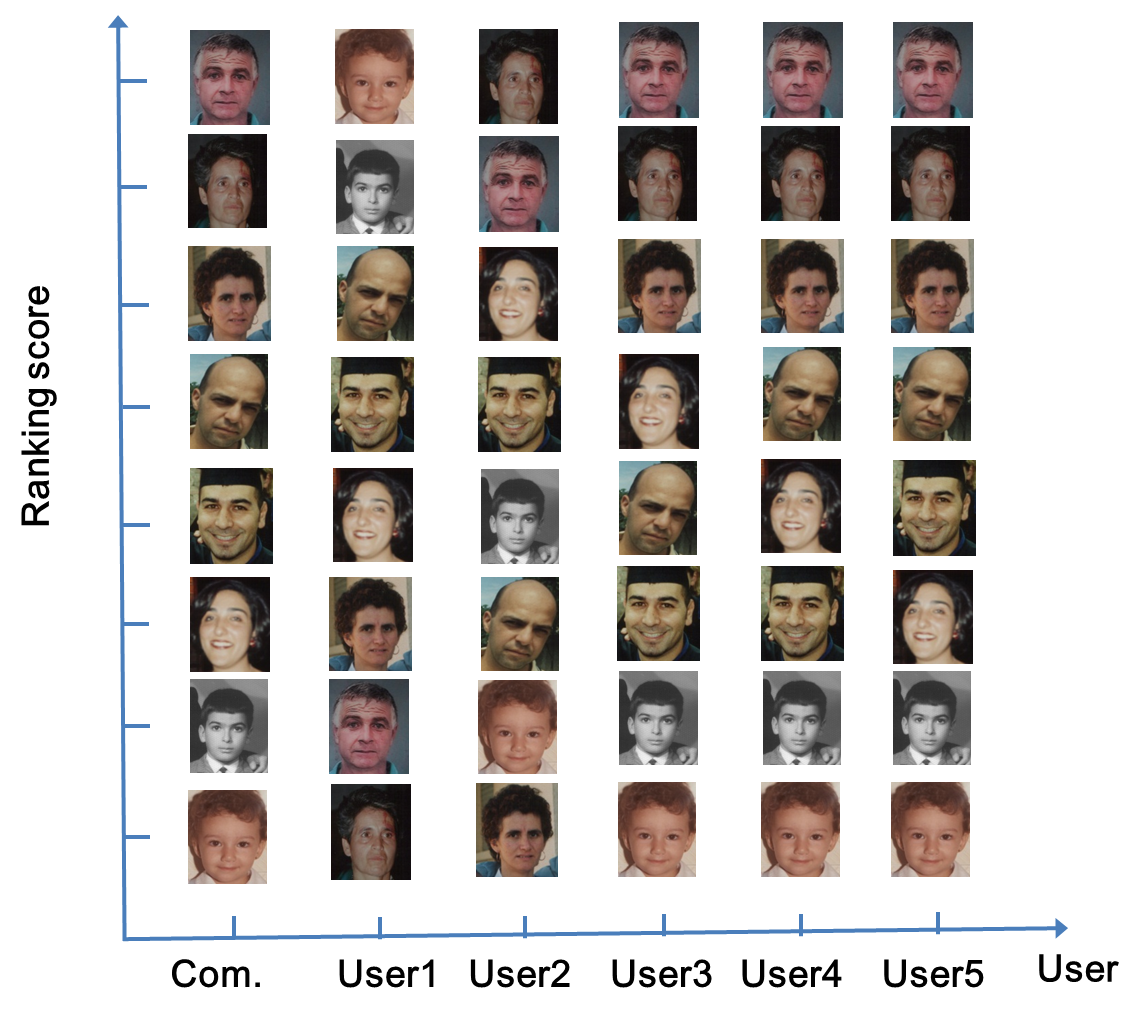
\includegraphics[width=0.8\linewidth]{1.png}
  \caption{An illustrative example on estimation of human ages, with the fixed effect of common ranking and random effects of user's personalized ranking. The faces in the first column are ordered according to a common ranking score aggregated from crowdsourced pairwise comparisons, while other columns are according to personalized rankings of different users. The ground truth ages in the first column, in a top-down order, are 46, 51, 36, 30, 25, 23, 10, and 2, respectively.} \label{introimage}
\end{center} \label{fig:age0}
\end{figure}

With the Internet and its associated explosive growth of information, individuals today in the world are facing with the
rapid expansion of multiple choices (e.g., which book to buy, which hotel to book, etc.). Inferring user's preference or utility over a set of alternatives has thus become an important
issue. Among various methods to infer user viewpoint/preference, crowdsourcing technology is becoming a new paradigm, which collects voting data from a large crowd or population on Internet and pursue some statistical preference aggregations. For example, the following platforms are frequently used by researchers to crowdsource voting data of participants: \href{https://www.mturk.com}{MTurk}, \href{http://www.innocentive.com/}{InnoCentive}, \href{http://crowdflower.com/}{CrowdFlower},~\href{http://www.crowdrank.net/}{CrowdRank}, and \href{http://www.allourideas.org/}{AllOurIdeas}, etc. A typical and perhaps the simplest scenario is the pairwise comparison experiment. Specifically,
there are a set of items to rank, and participants are asked to choose between various pairs among these items; the goal is to aggregate these pairwise comparisons
into a global consensus ranking that summarizes the preference of all users. We have seen that researchers exploit such a paradigm to evaluate the quality of multimedia content \cite{MM09}, predict image/video interestingness \cite{fu2014interestingness}, estimate ages from face pictures \cite{fu2015robust}, and rank taste of food \cite{jamieson2011active} etc.


However, different individuals might very well have distinct preferences, such that participants of the crowdsourced experiments might vote under different criteria or conditions. It might be misleading to merely look at a global consensus while ignoring personal diversity. For example Fig.\ref{fig:age0} shows an age estimation from photos that will be discussed in detail later in this paper. The majority is not always correct, as the common ranking by mistake thinks 46 older than 51! Moreover, even though {\tt User2} is largely deviated from the common ranking, it is noticeable that he/she makes correct judgements between the faces of year 46 and 51. So if one is looking for features that correctly predict the ages of these two particular faces, {\tt User2} is a better consultant than the majority. Particularly, {\tt User1} is clearly an adversarial voter, whose personalized ranking is largely against the common ranking reflecting the majority, so should be removed from a preference aggregation procedure.

Moreover, in crowdsourcing experiments, the participants are distributed over the Internet with a diverse environment. Even they might share the same preference or utility function in making choices, they might suffer various disturbances during the experiments. For example, i) one typically clicks one side more often than another. As some pairs are highly confusing or annotators get too tired, in these cases, some annotators tend to click one side hoping to simply raise their record to receive more payment; while for pairs with substantial differences, they click as usual. ii) some extremely careless annotators, or robots pretending to be human annotators, actually do not look at the instances and click one side all the time to quickly receive payment for work. Such a kind of behavior is called the annotator's position bias which has been studied in \cite{day1969position}.

These examples above suggest us that we have to take into account of user or annotator specific variations in a crowdsourced preference aggregation task.
As the classical social choice theory \cite{Arrow51} points out, preference aggregation toward a global consensus is doomed to meet the conflicts of interests. \emph{What is a suitable way to quantitatively analyze the conflicts of interests}?

In this paper, we pursue the Hodge-theoretic approach by \cite{Hodge} which decomposes the pairwise comparison data into three orthogonal components: the global consensus ranking, the local inconsistency as triangular cycles, and the global inconsistency as harmonic cycles. The latter two are both cycles, collectively decoding all the conflicts of interests in the data. Instead of the merely extracting from the data the global ranking component, often called \emph{HodgeRank} which has been introduced into the quality assessment of multimedia by \cite{tmm12}, we extend it here by including some annotator-specific random effects to further decompose the cycles. To decipher the sources of the conflicts of interests, we mainly consider two types of annotator-specific variations: annotator's personalized preference deviations from the common ranking which characterize multi-criteria in data, and annotator's position bias which deteriorates the quality of data. This results in a linear mixed-effects extension of HodgeRank, called Mixed-Effects HodgeRank here.

%In many other settings, we would like to look at
%those distinctions. For example, we might wish to provide personalized viewpoints, search results, or movie recommendations on a per user basis. A straightforward way is
%to build a linear model for each individual user based on
%the user's feedback on items. However, such linear model still suffers from the data sparsity
%issue, as it requires sufficient feedback examples for each individual user. Motivated by this observation,
%in recent years, some researchers propose collaborative filtering or low rank
%factorization model,
%which works by assuming that
%despite the diversity in the ranking lists from different users,
%there exist a small number of underlying intrinsic ranking
%functions such that all the ranking lists are derived from a
%linear combination of these intrinsic ranking functions (i.e., convergence behavior).
%It has been shown that collaborative filtering can produce high quality recommendations, but
%the performance degrades with the number of
%users and items.

To initiate a task of crowdsourced preference aggregation, we usually assume the majority of participants share a common preference interest and behave rationally, while deviations from that exist but are sparse. So a parsimonious model is assumed in this paper, with sparsity structure on personalized preference deviations and position biases. Due to the unknown amount of such sparse random effects in reality, it is natural to pursue a family of parsimonious models at a variety levels of sparsity. Algorithmically we adopt the Linearized Bregman Iteration, which is a simple iterative procedure generating a sequence of parsimonious models, evolving from the common global ranking in HodgeRank, to annotator's personalized ranking till a full model. Fig.\ref{fig:age0} is in fact a result of our algorithm. As the algorithm iterates, typically the abnormal annotators with large preference deviations and/or position biases appear early, and the annotators who behave normally appear at a later stage. In practice when the number of participants is large and sample size is relatively small, early stopping regularization is needed to prevent the overfitting in full model.

Equipped with such a new scheme, given a set of entities, we choose a
set of entity pairs and ask Internet crowds which entity is more preferable
in each pair. Based on the feedback we not only can derive the common preference on population-level, but also can estimate rapidly an annotator's large preference/utility deviation in an individual-level, and an abnormal annotator's position bias. Individual preference deviations from the population common ranking are helpful to understand different criteria among annotators when they judges, and especially to monitor the adversarial users. On the other hand, annotator's position bias is a helpful tool to monitor the quality of his/her voting data, through the mixing behavior that the annotator simply clicks one side of the pair in comparisons without paying attention to their contents. Such a statistical mixed-effects framework simultaneously considers both the fixed effect of common ranking as the HodgeRank and the random effects of annotator-specific variations, which, up to the author's knowledge, has not been seen in literature.

As a summary, our main contributions in this new framework are highlighted as follows:

\begin{itemize}
\item[(A)] A linear mixed-effects extension of HodgeRank including both the fixed effect of common ranking, and the random effects of annotator's preference deviation with position bias;
\item[(B)] A path of parsimonious estimates of the preference deviation and position bias at different sparsity levels, based on Linearized Bregman Iterations.
\item[(c)] Three kinds of losses (i.e. L2 loss, Bradley-Terry, Thurstone-Mosteller) in the dynamic Linearized Bregman Iterations scheme.
%\item[(C)] Extensive experimental validation based on one simulated and three real-world crowdsourced datasets.
\end{itemize}

This paper is an extension of our conference paper
\cite{mm16}, where only L2 loss is considered. Though it is much easier to solve and the Hodge Theory is adapted to the new inner product with orthogonal decomposition, it may lose some efficiency than Maximum likelihood methods. Therefore, in this paper, three kinds of losses (i.e. L2 loss, Bradley-Terry, Thurstone-Mosteller) are taken into consideration with detailed comparative analysis.

The remainder of this paper is organized as follows. Sec.\ref{sec:relatedwork} contains a review of related works. Then we systematically introduce the methodology for parsimonious mixed-effects HodgeRank estimation in Sec.\ref{sec:methodology}. Extensive experimental validation based on one simulated and three real-world crowdsourced datasets are demonstrated in Sec.\ref{sec:experiment}. Finally, Sec.\ref{sec:conclusion} presents the conclusive remarks.


\section{Related Work} \label{sec:relatedwork}

\subsection{Statistic Ranking Aggregation}

Statistical preference aggregation, in particular ranking or rating from pairwise comparisons,
is a classical problem which can be traced back to the $18^{th}$ century.
Various algorithms have been studied for this problem, including maximum
likelihood under a Bradley-Terry model
assumption, rank centrality (PageRank/MC3) \cite{negahban2012,dwork2001rank}, HodgeRank \cite{Hodge}
, and a pairwise variant of Borda
count \cite{de1781memoire} among others. In \cite{ICML14}, it shows that under a natural statistical model, where pairwise comparisons
are drawn randomly and independently from some
underlying probability distribution, the rank centrality (PageRank) and
HodgeRank algorithms both converge to an optimal ranking under
a ``time-reversibility" condition. However, PageRank is only able to aggregate the pairwise comparisons
into a global ranking over the items. HodgeRank not only provides us a mean to determine a global ranking under
various statistical models, but also measures the inconsistency of the global ranking obtained.

HodgeRank, as an application of combinatorial Hodge theory to the preference or rank aggregation problem from pairwise comparison data, was first introduced in~\cite{Hodge}, inspiring a series of studies in statistical ranking~\cite{hodge_l1,osting2013enhanced} and game theory~\cite{Parrilo11_gameflow}, in addition to traditional applications in fluid mechanics~\cite{Chorin93} and computer vision~\cite{Yuan09_hodge}, {etc}. It is a general framework to decompose paired comparison data on graphs, possibly imbalanced (where different video pairs may receive different number of comparisons) and incomplete (where every participant may only give partial comparisons), into three orthogonal components. In these components HodgeRank not only provides us a mean to determine a global ranking from paired comparison data under various statistical models (e.g., Uniform, Thurstone-Mosteller, Bradley-Terry, and Angular Transform), but also measures the inconsistency of the global ranking obtained. The inconsistency shows the validity of the ranking obtained and can be further studied in terms of its geometric scale, namely whether the inconsistency in the ranking data arises locally or globally. Local inconsistency can be fully characterized by triangular cycles, while global inconsistency involves cycles consisting nodes more than three, which may arise due to data incompleteness and once presented with a large component indicates some serious conflicts in ranking data. However through random graphs, we can efficiently control global inconsistency.

However, all of these methods have a major drawback: they aim to find one
ranking thus cannot
model the discrepancies across users. Therefore, in recent years, personalized ranking methods arise to fill in this gap.
This task can be seen as rank aggregation
analog to the standard collaborative filtering (CF) problem.
There
have been many CF algorithms, including Bayesian networks,
clustering models, and latent semantic models, etc. Recent algorithms
 for collaborative filtering are mostly based on matrix factorization \cite{salakhutdinov2008bayesian,rennie2005fast}.
  The key idea behind them is to find a low rank user rating matrix that best approximates the observed ratings. Most recently, the application of the nuclear norm approach to CF was first proposed by \cite{yi2013inferring}, which shows good empirical evidence for using such a nuclear
norm regularized based approach. The key difference between our
study and the low rank matrix collaborative filtering algorithms is that we assume the majority of voters share a fixed effect of common ranking while some annotators might deviate from that significantly. Such parsimonious model from population to individual is a natural fit for crowdsourcing scenarios.

\subsection{Linearized Bregman Iteration (LBI)}
Linearized Bregman Iteration (LBI) was firstly introduced in \cite{YODG08} in the literature of variational imaging and compressive sensing. It is well-known that LASSO estimators are always biased \cite{Fan2001}. On the other hand, \cite{OBG+05} notices that Bregman iteration may reduce bias, also known as contrast loss, in the context of Total Variation
image denoising. Now LBI can be viewed as a discretization of differential equations (inclusions), called \emph{Inverse Scale Spaces}, %\cite{burger2005nonlinear}
which may produce unbiased estimators under nearly the same model selection consistency conditions as LASSO \cite{osher2014}. %Furthermore, the idea of the linearized Bregman iteration is proposed \cite{Osher2008} to combine a fixed point iteration and the Bregman iteration in \cite{OBG+05, Yin08bregmaniterative}.

Beyond such a theoretical attraction, LBI is an extremely simple algorithm which combines an iterative gradient descent algorithm together with a soft thresholding. It is different to the well-known iterative soft-thresholding algorithm (ISTA) (e.g., \cite{Donoho95,fista} and references therein) which converges to the biased LASSO solution. To tune the regularization parameter in noisy settings, one needs to run ISTA with many different thresholding parameters and chooses the best among them; in contrast, LBI only runs in a single path and regularization is achieved by early stopping like boosting algorithms \cite{osher2014}, which may save the computational cost greatly and thus suitable for large scale implementation, e.g., distributive computation \cite{LBI_decentral}. %Therefore, in \cite{osher2014}, it studies noisy sparse signal recovery via a differential equation approach which may return an estimator that is both sign-consistent and bias-free. There are also distribution-based, depth-based, distance-based, density-based, and clustering method \cite{papadimitriou2003loci}, etc.
%



\section{Methodology}
\label{sec:methodology}

In this section, we systematically introduce the methodology
for parsimonious mixed-effects HodgeRank estimation. Specifically,
we first start from extending the HodgeRank to a linear mixed-effect model.
Then we present a simple iterative algorithm called Linearized Bregman Iterations to generate paths of parsimonious models at different sparsity levels.
Early stopping regularization is discussed in the end.

\subsection{Mixed-Effects HodgeRank on Graphs}


In crowdsourced pairwise comparison experiments, Let $V = \{1,2,\dots,n\}$ be the set of nodes and $E = \{(u,i,j): i,j\in V, u \in U\}$ be the set of edges, where $U$ is the set of all annotators. Suppose the pairwise ranking data is given as $y: E\rightarrow R$. $y_{ij}^u>0$ means $u$ prefers $i$ to $j$ and $y_{ij}^{u}\leq 0$ otherwise. The magnitude of $y_{ij}^u$ can represent the degree of preference and it varies in applications. The simplest setting is the binary choice, where
\begin{align}
y_{ij}^u=\left\{\begin{array}{cc}
                                                  1 & \mathrm{if} \ u \ \mathrm{prefers} \ i \ \mathrm{to} \ j, \\
                                                  -1 & \mathrm{otherwise}.
                                                \end{array}
                                                \right.
\label{eq:Y}
\end{align}

%In preference aggregation, it is natural to consider the following linear model:
%\begin{equation} \label{eq:linear}
%y_{ij}^u = \theta_i - \theta_j + \varepsilon_{ij}^\alpha
%\end{equation}
%where $\theta: V\to \mathbb{R}$ is some common score on $V$ and $\varepsilon_{ij}^u$ are independent noise of mean zero and fixed variance.
%
%Via HodgeRank,
%one benefits from the use of square loss L(x; y) = (x ?? y)2
%which leads to fast algorithms to find optimal global ranking
%x, as well as an orthogonal decomposition of the least square
%residue into local and global inconsistencies [4].
%

The general purpose of preference aggregation is to look for a global score $\theta\colon V\to \R$ such that
\begin{equation} \label{eq:ho_rank0}
\min_{\theta\in {\mathbb{R}}^{|V|}} \sum_{i,j,u} \omega_{ij}^u l(\theta_i - \theta_j, y_{ij}^u),
\end{equation}
where $l(x,y)\colon \R\times \R\to \R$ is a loss function, $\omega_{ij}^u$ denotes the confidence weights on $\{i,j\}$ made by rater $u$ (for simplicity, assumed to be $\omega_{ij}^u=1$ for the existing voting data), and $\theta_i$ ($\theta_j$) represents the global ranking score of item \emph{i} (\emph{j}, respectively). In HodgeRank, one benefits from the use of square loss $l(x,y)=(x-y)^2$ which leads to fast algorithms to find optimal global ranking $\theta$, which becomes one component of a general orthogonal decomposition of paired comparison data \cite{Hodge}, i.e.
\[ y= global\ ranking \oplus cycles, \]
where the component \emph{cycles} can be further decomposed into
\[cycles = local\ cycles \oplus global\ cycles. \]

Local cycles are triangular cycles, e.g. $i \succ j \succ k\succ i $; while global cycles, also called harmonic cycles, are loops involving nodes more than three (e.g. $i \succ j \succ k \succ...\succ i$) and typically traversing all nodes in the graph. These cycles may arise due to conflicts of interests in ranking data. Therefore to analyze the statistical models of cycles is crucial to understand the conflicts of interests.

In crowdsourcing scenarios, the conflicts of interests are mainly due to two kinds of sources: the multi-criteria adopted by different annotators when they compare items in $V$; the abnormal behavior of annotators in the experiments, e.g. simply clicking one side of the pair when they got bored, tired, or distracted. To quantitatively characterize these effects, we propose the following model of cycles
\[ cycles = personalized\ ranking + position\ bias + noise. \]

%\textcolor{red}{From Hodgerank to LME, it is a little bit difficult for me.}
%\subsection{Linear Mixed Effects (LME) Models}
To be specific, together with the global ranking component in HodgeRank, we consider the following linear mixed effects model for annotator's pairwise ranking:
\begin{equation} \label{eq:linear}
y_{ij}^u = (\theta_i+\delta_i^u) - (\theta_j+\delta_j^u) + \gamma^u + \varepsilon_{ij}^u,
\end{equation}
where
\begin{itemize}
\item $\theta_i$ is the common global ranking score, as a fixed effect;
\item $\delta_i^u$ is the annotator's preference deviation from the common ranking $\theta_i$ such that $\theta_i^u:=\theta_i + \delta_i^u$ becomes annotator $u$'s personalized ranking score, as a random effect;
\item $\gamma^u$ is an annotator's position bias, which captures the careless behavior by clicking one side during the comparisons;
\item $\varepsilon_{ij}^u$ is the random noise which is assumed to be independent and identically distributed with zero mean and being bounded.
\end{itemize}

Putting in matrix form, \eqref{eq:linear} becomes
\begin{equation} \label{eq:linear-matrix}
y = d\theta + X\beta + \varepsilon,
\end{equation}
where $d\in \R^{|E| \times |V|}$ satisfies $d\theta(u,i,j) = \theta_i-\theta_j$, $\beta = [\delta, \gamma] \in R^{(|V|+1)|U|}$ and $X =[D,A]$, where $D \in \R^{|E| \times |V| |U|} $ satisfies $D\delta(u,i,j) = \delta^u_i-\delta^u_j$ and $A \in \R^{|E| \times |U|}$ satisfies $\gamma(u,i,j) = \gamma^u$.

Here $\theta$ is population-level parameter which indicates some common score on $V$.  In crowdsourcing studies, as the data vary greatly
across individual annotators, we thus allow each annotator to have personalized
parameters $\theta^u$. These personalized parameters can be obtained by adding some
random effects $\delta^u$ to the population parameter $\theta$, representing individual deviations from the population behavior. Besides, $\gamma^u$ measures an annotator's position bias, i.e. the tendency of $u$ always clicking one side in paired comparison experiments. Under the random design of pairwise comparison experiments, a candidate should be placed on the left or the right randomly, so the position should not affect the choice of a careful annotator. However, some annotator might get confused, tired or distracted in experiments, such that he/she always clicks one side during some periods in experiments. Such a type of position bias captures a kind of noise in data not included in the zero mean $\varepsilon$ and may severely deteriorates the quality of data. The remainder $\varepsilon_{ij}^u$ measures the random noise in sampling which is of zero mean and bounded (hence subgaussian).

\subsection{Parsimonious Paths with Linearized Bregman Iteration}

In crowdsourced preference aggregation scenarios with good controls, it is natural to assume a parsimonious model. In such a model, the majority of annotators carefully follows the common behavior governed by the fixed effect parameter $\theta$, while only a small set of annotators might have nonzero personalized deviations and abnormal behavior in position bias. This amounts to assume that parameter $\delta^u$ to be group sparse, i.e. $\delta_i^u$ vanishes for all $i$ simultaneously, and $\gamma^u$ to be sparse as well, i.e. zero for most of careful annotators. Such a sparsity pattern motivates us to consider the following penalty function with a mixture of LASSO ($L_1$) penalty on $\gamma$ and group LASSO penalty on $\delta$:

%To learn a sparse model, penalty functions are often used, such as $L_1$-penalty(Lasso) and group lasso penalty. In this particular model, we need $L_1$-penalty on $\gamma$ and group lasso penalty on $\delta$:
\begin{equation}\label{eq-penalty}
P(\beta) = \|\gamma\|_1 + \sum_{u}\|\delta^u\|_2, \beta=(\delta,\gamma).
\end{equation}
%Since $|\gamma^u| = \sqrt{(\gamma^u)^2} =  \|\gamma^u\|_2$, this mixed penalty can also be regarded as simple group penalty with each $\gamma^u$ as a group.

{\begin{remark}
Usually a normalization factor $\sqrt{n}$ is used before a group lasso penalty $\|\delta^u\|_2$, where $n$ is the group size of $\delta^u$. But here all the $\delta^u$ have the same group size, and $\|D^u\|_F = \sqrt{2}\|A^u\|_F$, so the column norm of $D^u$ is on average $\frac{\sqrt{2}}{\sqrt{n}}$ times of $\|A^u\|_F$, this basically cancels out the factor $\sqrt{n}$. So here we just use this simple formula.
\end{remark}

Following the square loss in HodgeRank, the Euclidean distance (mean square error) in $R^{E}$ can be used for the total loss function:
\begin{equation}\label{eq-loss}
L(\theta,\beta) = \frac{1}{2m}\|y - d\theta - X\beta\|_2^2.
\end{equation}

The following Linearized Bregman Iterations (LBI) give rise to a sequence of parsimonious (sparse) models:
\begin{subequations}\label{eq:lbi0}
\begin{align}
\theta^{k+1} & = \theta^k - \alpha \kappa  \nabla_\theta L(\theta^k,\beta^k) \label{eq:lbi0-a}\\
z^{k+1} & = z^k - \alpha \nabla_\beta L(\theta^k,\beta^k), \label{eq:lbi0-b}\\
 \beta^{k+1} &=\kappa \cdot {\prox}_{P}(z^{k+1}), \label{eq:lbi0-c}
\end{align}
\end{subequations}
where $\beta^0 = 0$, $\theta^0 = \arg \min_{\theta} L(\theta,0)$, and variable $z$ is an auxiliary parameter used for gradient descent, $z = \rho+\beta/\kappa, \rho \in \partial P(\beta)$. Besides,
the proximal map associated with the penalty function $P$ is given by
\[ \prox_P(z) = \arg\min_{v \in R^{(|V|+1)|U|}} \left( \frac{1}{2}\| v - z\|^2 + P(z) \right ). \]

The Linearized Bregman Iteration \eqref{eq:lbi0} generates a path of global ranking score estimators $\theta^k$ and sparse estimators for preference deviation and position bias, $\beta^k=(\delta^k,\gamma^k)$. It starts from the common HodgeRank as $\theta^0 = \arg \min_{\theta} L(\theta,0)$, and evolves into parsimonious mixed effect models with different levels of sparsity until the full model, often overfitted. To avoid the overfitting, early stopping regularization is required to find an optimal tradeoff between the model complexity and in-sample error. For more details, we refer the readers to see \cite{osher2014} and references therein. In this paper, we find that cross validation works to find the early stopping time that will be discussed in Sec.\ref{sec:cv}.
%\[ t_{cv}:=\inf\{k\alpha: \mbox{$(\theta^k,\beta^k)$ minimizes the validation error}\},\]
% as what we did in the experimental section below.

The Linearized Bregman algorithm was firstly introduced in \cite{OBG+05} as a scalable algorithm for large scale image restoration with TV-regularization. It has several advantages than the widely used LASSO-type convex regularizations. First of all, it is simpler than LASSO in generating the sparse regularization paths: instead of a parallel run of several optimization problem over a grid of regularization parameters, a single run of LBI generates the whole regularization path. LBI is thus desired in dealing with big problems. Moreover, it can be less biased than LASSO as if nonconvex regularizations \cite{FanLi01}. In fact, it is shown recently in \cite{osher2014} that as $\kappa\to \infty$ and $\alpha_t\to 0$, the limit dynamics of Linearized Bregman Iterations in sparse linear regression with LASSO ($L_1$) penalty may achieve the model selection consistency under nearly the same condition as LASSO yet return the unbiased Oracle estimator, while the LASSO estimator is well-known biased.

% A traditional way to learn the model is to solve the following optimization problem:
%\begin{equation}\label{eq:lasso}
%\min_{\theta,\beta} L(\theta,\beta) + \lambda P(\beta)
%\end{equation}
%with the tuning parameter $\lambda$. However, as figured in \cite{FanLi01}, such a convex regularization approach is biased and they used non-convex penalty instead to reduce bias. Also \cite{OBG+05} introduces a new method to solve the bias problem, Linearized Bregman Iteration (LBI).

%Here we first introduce the LBI algorithm for universal Loss function $L(\theta,\beta)$ and Penalty function $P(\beta)$:
%\begin{algorithm}
%\caption{Linearized Bregman Algorithm.}\label{alg-LBI}
%\textbf{Input:} Loss function $L(\theta,\beta)$, Penalty function $P(\beta)$, damping factor $\kappa$, step size $\alpha$.\\
%\textbf{Initialize:} $\beta^0 = 0,\theta^0 = \arg \min_{\theta} L(\theta,0),\rho^0=0,t^0=0$.\\
%{\textbf{for $k=0,\dots,K$ do}
%\begin{enumerate}
%\item $\theta^{k+1} = \theta^k - \kappa\alpha\nabla_{\theta}L(\theta^k,\beta^{k})$. \label{alg1-step1}
%\item $\rho^{k+1}+\beta^{k+1}/\kappa  = \rho^{k}+\beta^{k}/\kappa - \alpha\nabla_{\beta}L(\theta^k,\beta^{k}), ~~ \rho^{k+1} \in \partial P(\beta^{k+1})$.\label{alg1-step2}
%\item $t^{k+1} = (k+1)\alpha$.
%\end{enumerate}
%\textbf{end for}}\\
%\textbf{Output:} Solution path $\{t^k, \theta^k,\beta^k\}_{k= 0,1,\dots,K}$.
%\end{algorithm}

Here we give some remarks on the implementation details of the Linearized Bregman Iterations \eqref{eq:lbi0}.
\begin{itemize}
\item The parameter $\kappa$ determines the bias of the sparse estimators, a bigger $\kappa$ leading to the less biased ones. The parameter $\alpha$ is the step size which determines the precise of the path, with a large $\alpha$ rapidly traversing a coarse grained path. However one has to keep $\alpha \kappa$ small to avoid possible oscillations of the paths, e.g. $\alpha \kappa \|X^T X\|_2/m<2$. The default choice in this paper is $\alpha  = \frac{m}{\kappa\|X^TX\|_2}$ as a tradeoff between performance and computation cost.
\item The step \eqref{eq:lbi0-a} can also be replaced by $$\theta^{k+1}  = \arg\min_{\theta}L(\theta,\beta^k)$$ if it is easy to solve.
\item Now we turn to simplify the third step \eqref{eq:lbi0-c} with an explicit formula for the proximal map with the particular penalty function defined in Eq. (\ref{eq-penalty}). Recovering $\beta^{k+1}$ from $z^{k+1}$ is equivalent to the following group shrinkage on each group component of $\beta$, i.e. $\gamma^u$ and $\delta^u$:
\begin{eqnarray}
\beta^{k+1} &=& \kappa \mathbf{Shrinkage}(z^{k+1})\\
&\triangleq &\left\{
\begin{aligned}
\delta^{u,k+1} &= \kappa\max(0,1-1/\|z_{\delta^u}\|_2)z_{\delta^u} \nonumber \\
\gamma^{u,k+1} &= \kappa\max(0,1-1/|z_{\gamma^u}|)z_{\gamma^u} \nonumber \\
\end{aligned}
\right.
\end{eqnarray}
\end{itemize}

%Let $z^k =  \beta^{k} + \rho^{k}/\kappa$, then it becomes $z^{k+1} = z^{k} - \alpha\nabla_{\beta}L(\theta^{k+1},\beta^{k})$. To recover $\beta^{k+1}$ from $z^{k+1}$, we need further calculation on the sub-gradient of group lasso penalty.
%\textbf{Property:} Suppose $x \in \R^{p}$, then
%\begin{equation}
%\partial \|x\|_2 = \left\{
%\begin{aligned}
% x/\|x\|_2, ~~&if~\|x\|_2>0\\
% \{\rho: \|\rho\|\le1\},~~&else\\
%\end{aligned}
%\right.
%\end{equation}
%Let $\rho$ is the sub-gradient of $\|x\|_2$, i.e. $\rho \in \partial \|x\|_2$ and $z = \rho+x/\kappa$, then
%\begin{equation}
%x = \kappa\max(0,1-1/\|z\|_2)z
%\end{equation}
%We will call it group shrinkage following. When $p=1$, it degenerates to soft-shrinkage.

Now we are ready to give the following Linearized Bregman Algorithm for our Mixed-Effects HodgeRank as
\begin{algorithm}
\caption{LBI for ME-HodgeRank}\label{alg-LBI-LME}
\textbf{Input:} Data $(d,X,y)$, damping factor $\kappa$, step size $\alpha$.\\
\textbf{Initialize:} $\beta^0 = 0,\theta^0 = (d^Td)^{-1}d^Ty,z^0=0,t^0=0$.\\
{\textbf{for $k=0,\dots,K$ do}
\begin{enumerate}
\item $\theta^{k+1} = (d^Td)^{-1}d^T(y - X\beta^k)$. \label{alg2-step1}
\item $z^{k+1}  =z^{k} + \frac{\alpha}{m} X^T(y - d\theta^k - X\beta^k)$.\label{alg2-step2}
\item $\beta^{k+1} = \kappa\mathbf{Shrinkage}(z^{k+1})$
\item $t^{k+1} = (k+1)\alpha$.
\end{enumerate}
\textbf{end for}}\\
\textbf{Output:} Solution path $\{t^k, \theta^k,\beta^k\}_{k= 0,1,\dots,K}$.
\end{algorithm}

% \textbf{Remark:}  In Alg. \ref{alg-LBI-LME}, the parameter $\kappa$ is actually A bigger $\kappa$ means less bias but more computation cost.
\subsection{General Linear Model for Binary Data} \label{sec:glm}
For binary data, the linear model \eqref{eq:linear} may be not a proper interpreter, even though it still works in many datasets. A more interpretable model is General Linear Model(GLM) for binary data:
\begin{align}\label{eq:glm}
P(y^u_{ij} = 1) &= 1-P(y^u_{ij}=-1) \nonumber\\
&= \Phi((\theta_i+\delta_i^u) - (\theta_j+\delta_j^u) + \gamma^u)
\end{align}
\eqref{eq:glm} where $\Phi(t)$ is a symmetric cumulative distribution function(CDF). When $\Phi(t) = \frac{1}{1+e^{-t}}$, it becomes Bradley-Terry model and $\Phi(t) = \frac{1}{\sqrt{2\pi}}\int_{-\infty}^{t}e^{-x^2/2}dx$ indicates Thurstone-Mosteller model.

Under GLM assumption, a natural estimation method is to minimize the negative log-likelihood:
\begin{equation}\label{eq:likelihood}
L(\theta,\beta) = -\frac{1}{m}\sum_{i,j,u}\log\Phi(y^u_{ij}((\theta_i+\delta_i^u) - (\theta_j+\delta_j^u) + \gamma^u)).
\end{equation}
Here we use the fact $\Phi(-t) = 1-\Phi(t)$. Plug it in \eqref{eq:lbi0}, the corresponding LBI can be used to estimate a sequence of parsimonious sparse models for GLM.

\begin{algorithm}
\caption{LBI for ME-GLM}\label{alg-LBI-GLM}
\textbf{Input:} Data $(d,X,y)$, damping factor $\kappa$, step size $\alpha$.\\
\textbf{Initialize:} $\beta^0 = 0,\theta^0 = 0,z^0=0,t^0=0$.\\
{\textbf{for $k=0,\dots,K$ do}
\begin{enumerate}
\item $r^k = y.*(d\theta^k + X\beta^k)$.
\item $\theta^{k+1} = \theta^k +  \frac{\alpha\kappa}{m}   d^T(\phi(r^k).*y./\Phi(r^k))$.
\item $z^{k+1}  =z^{k} + \frac{\alpha}{m} X^T(\phi(r^k).*y./\Phi(r^k))$.
\item $\beta^{k+1} = \kappa\mathbf{Shrinkage}(z^{k+1})$
\item $t^{k+1} = (k+1)\alpha$.
\end{enumerate}
\textbf{end for}}\\
\textbf{Output:} Solution path $\{t^k, \theta^k,\beta^k\}_{k= 0,1,\dots,K}$.
\end{algorithm}
Alg \ref{alg-LBI-GLM} is the detailed algorithm, where $.*$ and $./$ means entry-wise multiplication/division and $\phi(t) = \Phi'(t)$ is the probability distribution function corresponding to $\Phi(t)$. Here $\phi(t) =  \frac{e^t}{(1+e^{t})^2}$ corresponds to Bradley-Terry model and $\phi(t) = \frac{1}{\sqrt{2\pi}}e^{-x^2/2}$ for Thurstone-Mosteller model.


\subsection{Early Stopping Regularization} \label{sec:cv}
The Alg.\ref{alg-LBI-LME} actually returns a solution path with many estimators of different sparsity. So we need to find an optimal stopping time among $t^k=\alpha k$ to choose some best estimators and avoid overfitting. Here we sketch the procedure of cross-validation to choose the optimal stopping time:
\begin{itemize}
\item Given the training data, fix $\kappa$ and $\alpha$, then split the data into $K$ folds. Then choose a list of parameter $t$.
\item \textbf{for $k=1,\dots,K$ do}
	\begin{enumerate}
	\item Run Alg.\ref{alg-LBI-LME} on the training data except $k$-th fold to get the solution path.
	\item For pre-decided parameter list of $t$, use a linear interpolation to get $(\theta(t),\beta(t))$.
	\item On the $k$-th fold of training data, use the estimator $(\theta(t),\beta(t))$ to predict, and then compute prediction error.
	\end{enumerate}
	\textbf{end for}
\item  Return the optimal $t_{cv}$ with minimal average prediction error.
\end{itemize}
\textbf{Remark:} Because the Alg.\ref{alg-LBI-LME} only returns the estimator at discrete $\{t^k\}$ and may not contain the pre-decided parameter $t$, so we use a linear interpolation of the nearest two estimator $(\theta^{k},z^{k})$ and $(\theta^{k+1},z^{k+1})$ to approximate $(\theta(t),z(t))$. $\beta(t)$ is further obtained by using $\mathbf{Shrinkage}(z(t))$.




\begin{figure*}[t]
% \renewcommand{\captionfont}{\scriptsize \bfseries}
 \begin{center}
  \subfigure[Annotators with personalized ranking detected by L2 loss]{
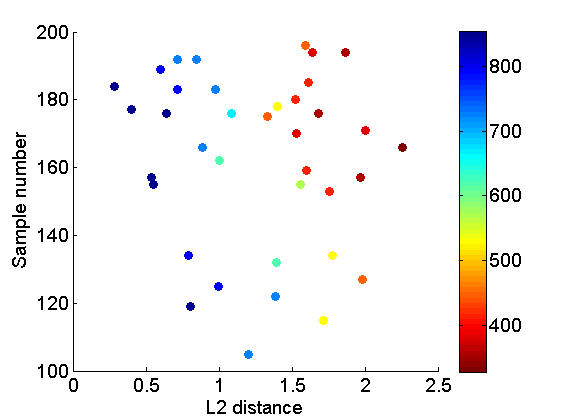
\includegraphics[width=0.3\textwidth]{simu_l2_preference_dot.png}\label{simulated1}}
\subfigure[Annotators with personalized ranking detected by Bradley-Terry]{
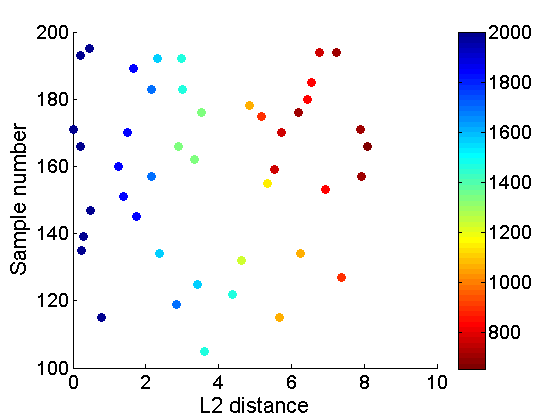
\includegraphics[width=0.3\textwidth]{simu_model1_preference_dot.png}\label{simulated1_model1}}
\subfigure[Annotators with personalized ranking detected by Thurstone-Mosteller]{
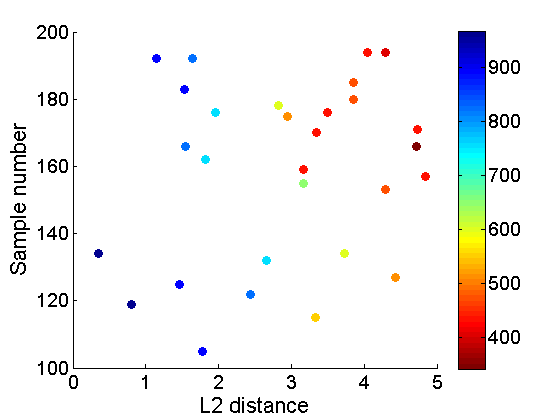
\includegraphics[width=0.3\textwidth]{simu_model2_preference_dot.png}\label{simulated1_model2}}
   \subfigure[Position-biased annotators detected by L2 loss]{
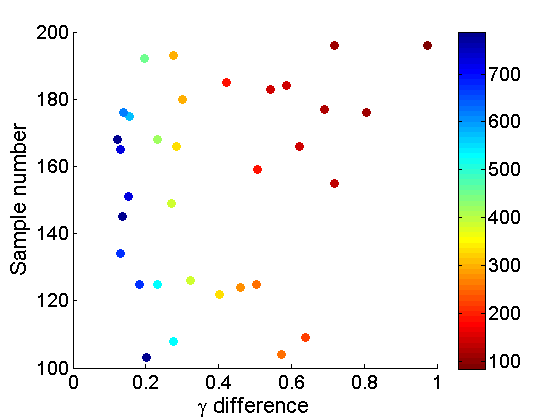
\includegraphics[width=0.3\textwidth]{simu_l2_position_dot.png}\label{simulated2}}
   \subfigure[Position-biased annotators detected by Bradley-Terry]{
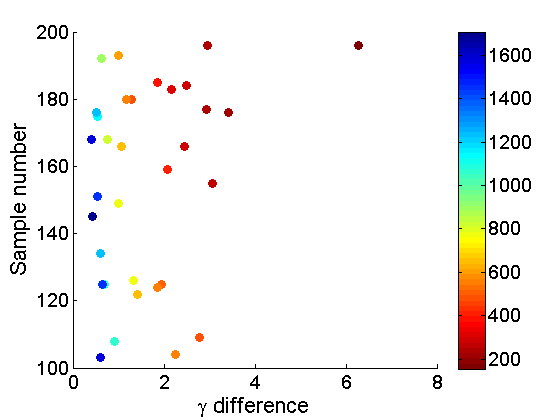
\includegraphics[width=0.3\textwidth]{simu_model1_position_dot.png}\label{simulated2_model1}}
   \subfigure[Position-biased annotators detected by Thurstone-Mosteller]{
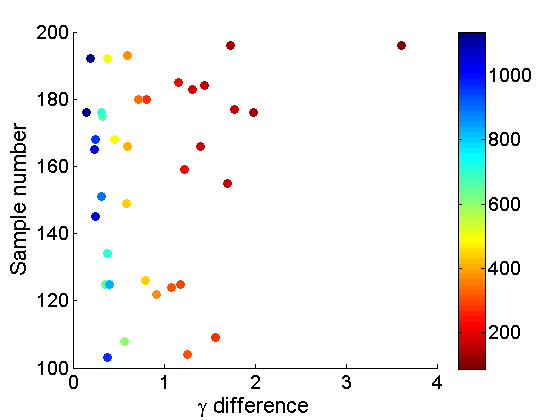
\includegraphics[width=0.3\textwidth]{simu_model2_position_dot.png}\label{simulated2_model2}}
  \caption{Annotators with personalized ranking and position bias detected in simulated data.}
\end{center}
\end{figure*}


\section{Experiments}\label{sec:experiment}

In this section, four examples are exhibited with both
simulated and real-world data to illustrate the validity of
the analysis above and applications of the methodology proposed.
The first example is with simulated data while the
latter three exploit real-world data collected by crowdsourcing.

\subsection{Simulated Study}
\textbf{Settings} We validate the proposed algorithm on simulated data labeled by 100 annotators.
Specifically, we first generate the true $\theta_i \sim \N(0,1)$.
Then each annotator has a probability $p_1 = 0.4$ having a nonzero $\gamma^u$ and a probability $p_2 = 0.4$ having a nonzero $\delta^u$.
Those nonzero $\gamma^u$ is drawn randomly from $\N(0,2^2)$. And each entry $\delta_i^u$ of nonzero $\delta^u$ is drawn randomly from $\N(0,s^2)$ with $s \sim \mathbb{U}(0,3)$.
At last, we draw $N^u$ samples for each user randomly with binary response $y^u_{ij}$ following the model $P(y^u_{ij} = 1) = \Phi((\theta_i+\delta_i^u) - (\theta_j+\delta_j^u) + \gamma^u)$, where $\Phi(t) = 1/(1+e^{-t})$.
 The sample number $N^u$ uniformly spans in $[N_1,N_2] = [100,200]$. Here we choose $n=|V|=16$, which is consistent with the first real-world dataset.  Finally, we obtain a multi-edge graph with 15,067 pairwise comparisons annotated by 100 annotators.





\textbf{Results} Fig.\ref{simulated1}, \ref{simulated1_model1}, and \ref{simulated1_model2} show the annotators exhibiting personalized preferences selected via three loss cases, where each color dot represents one annotator. The optimal $t$ obtained via cross-validation is shown in Fig.\ref{simulated3}. The scores derived from each user are denoted as $\hat{\theta}^u$ and the common ranking as $\hat{\theta}$. The X-axis represents the $L_2$-distance between each user's personalized ranking and the common ranking, $\|\hat{\theta}^u-\hat{\theta}\|$. The Y-axis counts the number of pairwise comparisons each user provides.
Clearly one can see the larger the $L_2$-distance and sample size, the more earlier this user is treated as one with personalized ranking (from color red to blue). This indicates that users jumped out earlier are those with large deviation from the population's opinion and a big sample size indicating a high confidence. Similar results of position-biased user are illustrated in Fig.\ref{simulated2}, \ref{simulated2_model1}, and \ref{simulated2_model2} in which the X-axis ($\gamma$ difference) represents the absolute difference of $\gamma$ between each user and the population.


Finally, to see whether our proposed method in three loss cases could provide more precise preference function for users by introducing individual-specific parameters (i.e., $\delta$ and $\gamma$), we split the data into training set ($70\%$ of the total pairwise comparisons) and testing set (the remaining $30\%$). To ensure the statistical
stability, we repeat this procedure 20 times. Tab.\ref{simulatedresult} shows the experimental results of the proposed mixed-effects model compared with HodgeRank, which indicates that our method exhibits smaller test error (i.e. mismatch ratio) due to its
parsimonious property. Besides, it is worth mentioning that L2 loss could exhibit similar performance with Bradley-Terry and Thurstone-Mosteller models which are particular suitable for binary data in most cases.





\begin{figure*}
% \renewcommand{\captionfont}{\scriptsize \bfseries}
 \begin{center}
  \subfigure[L2 Loss]{
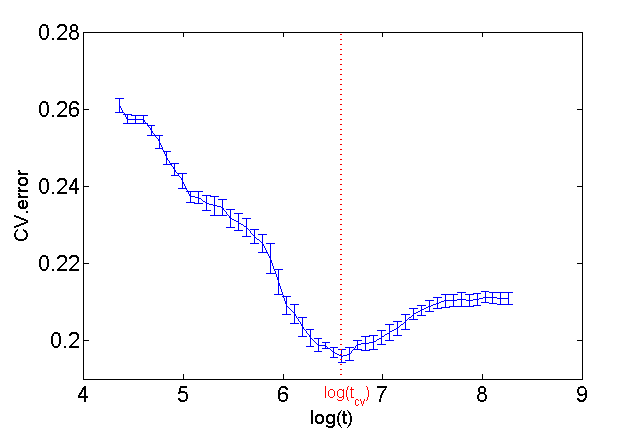
\includegraphics[width=0.3\textwidth]{simu_l2_error.png}}
   \subfigure[Bradley-Terry]{
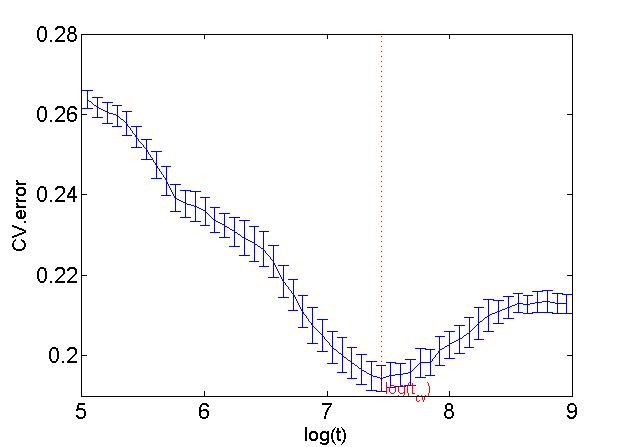
\includegraphics[width=0.28\textwidth]{simu_model1_error.png}}
\subfigure[Thurstone-Mosteller]{
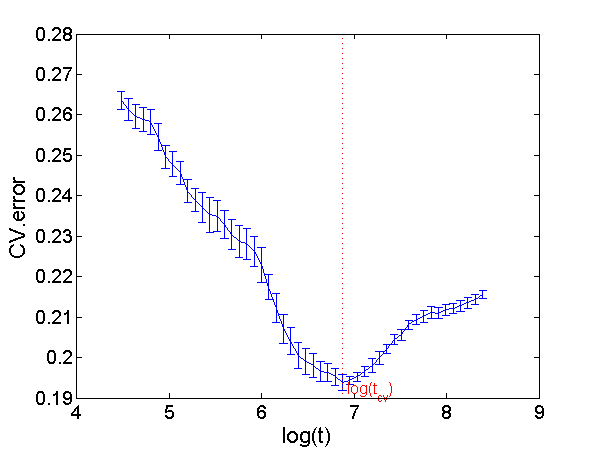
\includegraphics[width=0.26\textwidth]{simu_model2_error.png}}
  \caption{Optimal $t$ with minimal average prediction error in simulated data.} \label{simulated3}
\end{center}
\end{figure*}

%
%\begin{figure}[t]
%%\setlength{\belowcaptionskip}{-22pt}
%%\setlength{\abovecaptionskip}{5pt}
%%\renewcommand{\captionfont}{\scriptsize \bfseries}
% \begin{center}
%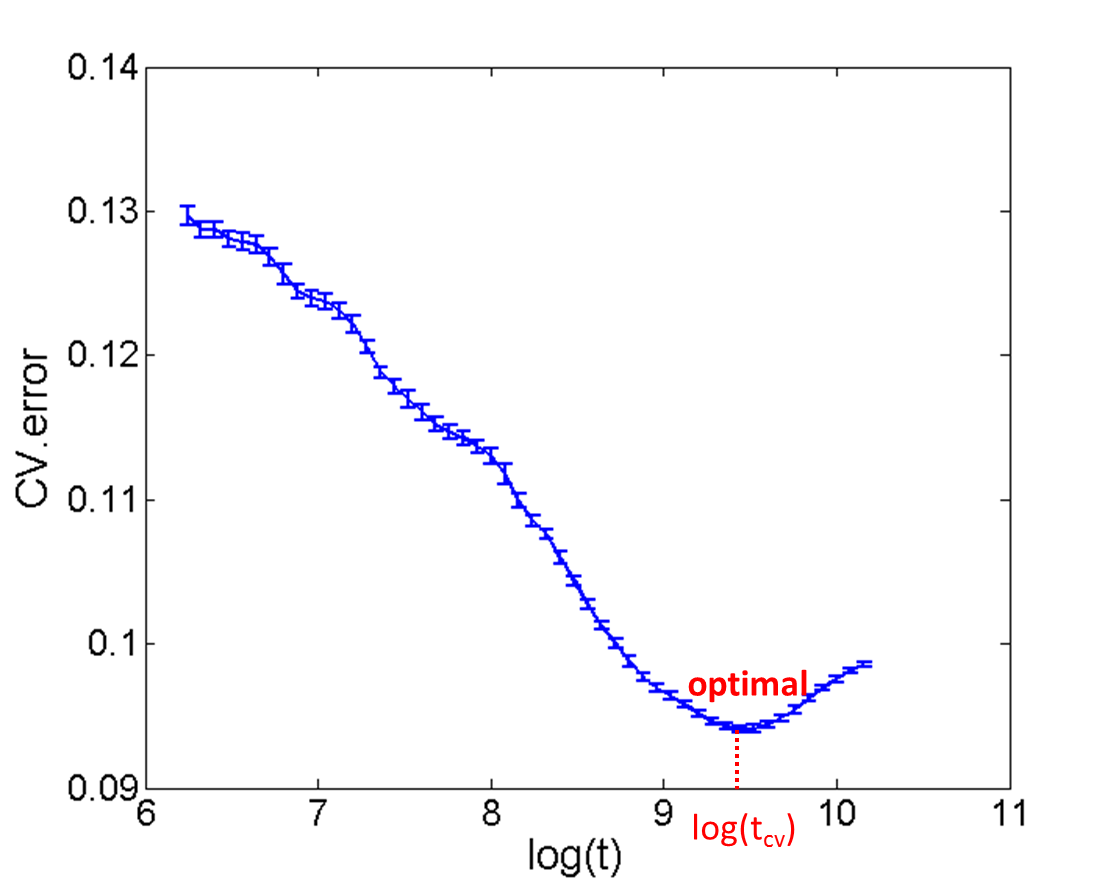
\includegraphics[width=0.65\linewidth]{cv.png}
%  \caption{Optimal $t$ with minimal average prediction error in simulated data.} \label{simulated3}
%
%\end{center}
%\end{figure}




\begin{table}\caption{\label{simulatedresult} HodgeRank vs. Mixed-effects model on test error (i.e. mismatch ratio) in simulated data.}
\centering
\begin{tabular}{lllll}
 \hline     &min  &mean &max &std\\
 \hline  HodgeRank     &0.2573    &0.2645    &0.2760    &0.0051 \\
\hline  L2 Loss    &0.1902    &\textcolor{red}{0.1983}    &0.2063    &0.0044  \\
\hline Bradley-Terry    &0.1930    &\textcolor{red}{0.1980}    &0.2053    &0.0034 \\
\hline Thurstone-Mosteller    &0.1912    &\textcolor{red}{0.1981}    &0.2056    &0.0042
  \\
 \hline
 \end {tabular}
\end{table}




\subsection{Human Age}



\begin{figure}[h]
%\setlength{\belowcaptionskip}{-22pt}
%\setlength{\abovecaptionskip}{5pt}
%\renewcommand{\captionfont}{\scriptsize \bfseries}
 \begin{center}
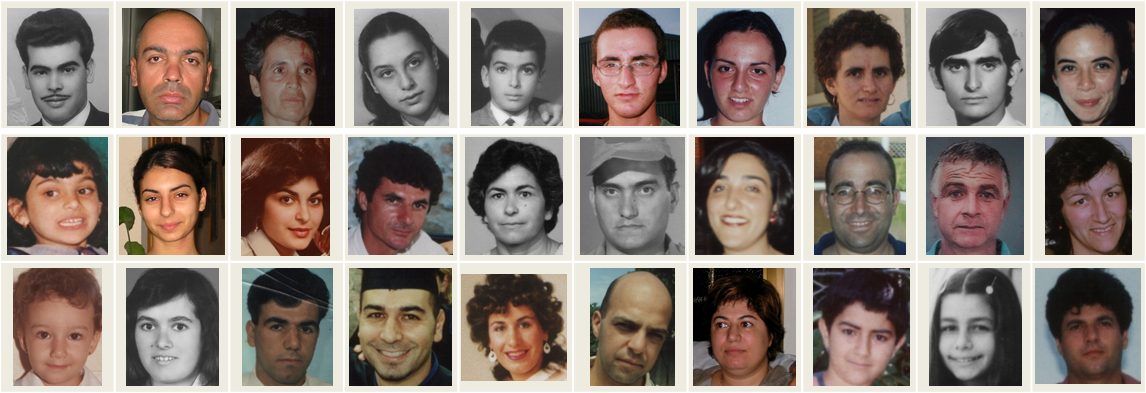
\includegraphics[width=0.8\linewidth]{agedataset.png}
  \caption{Images in Human age dataset.} \label{agedataset}
\end{center}
\end{figure}


\begin{table}[h]\caption{\label{tab:age} HodgeRank vs. Mixed-effects model in Human age dataset.}
\centering
\begin{tabular}{lllll}
 \hline     &min  &mean &max &std\\
 \hline  HodgeRank     &0.1997    &0.2104    &0.2202    &0.0050 \\
\hline  L2 Loss     &0.1478    &\textcolor{red}{0.1569}    &0.1653    &0.0055  \\
\hline Bradley-Terry  &0.1191    &\textcolor{red}{0.1255}    &0.1341    &0.0046 \\
\hline Thurstone-Mosteller    &0.1214    &\textcolor{red}{0.1283}    &0.1356    &0.0042  \\
 \hline
 \end {tabular}
\end{table}




\begin{figure*}
% \renewcommand{\captionfont}{\scriptsize \bfseries}
 \begin{center}
  \subfigure[L2 Loss]{
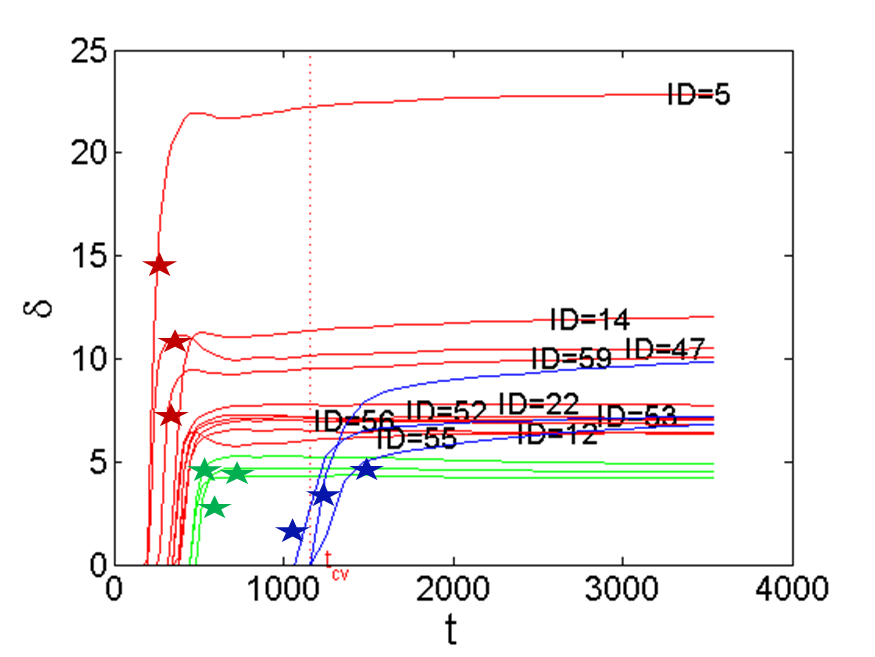
\includegraphics[width=0.3\textwidth]{L2-preference-age.png}}
   \subfigure[Bradley-Terry]{
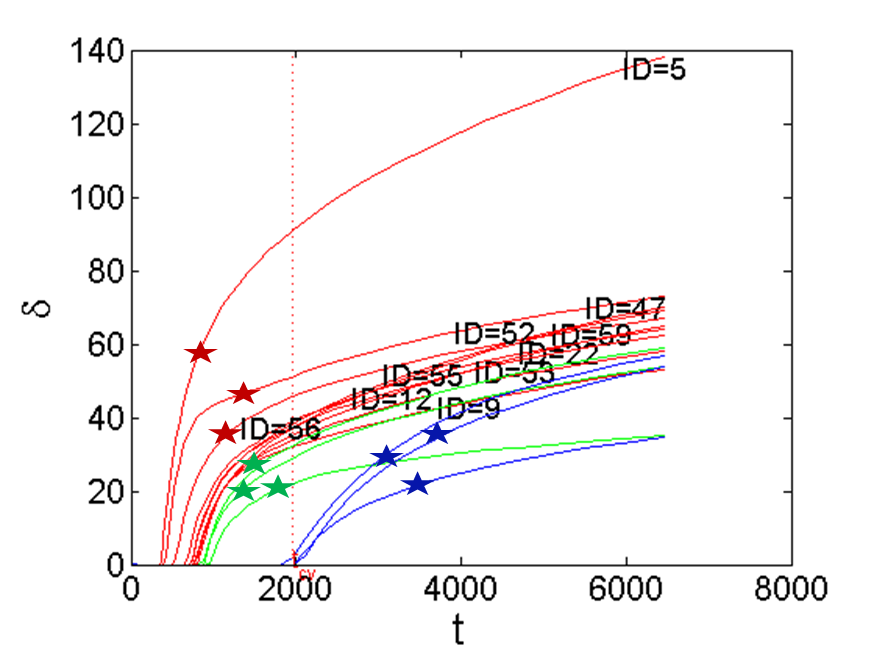
\includegraphics[width=0.3\textwidth]{model1-preference-age.png}}
\subfigure[Thurstone-Mosteller]{
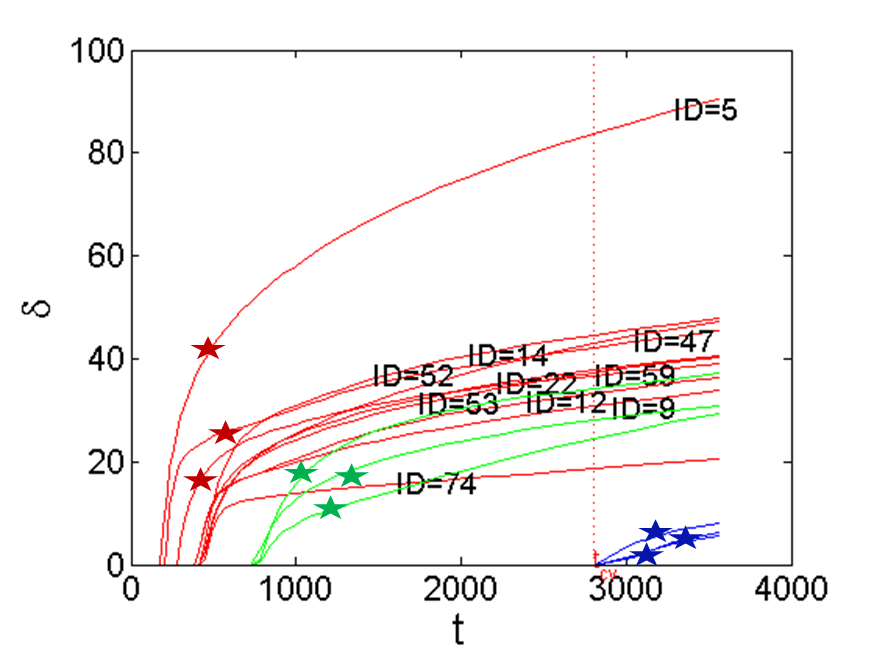
\includegraphics[width=0.3\textwidth]{model2-preference-age.png}}
  \caption{Top 10 (marked with red color) annotators with personalized ranking in Human age dataset.}\label{fig:agepreferencepath}
\end{center}
\end{figure*}




\begin{figure*}
% \renewcommand{\captionfont}{\scriptsize \bfseries}
 \begin{center}
  \subfigure[L2 Loss]{
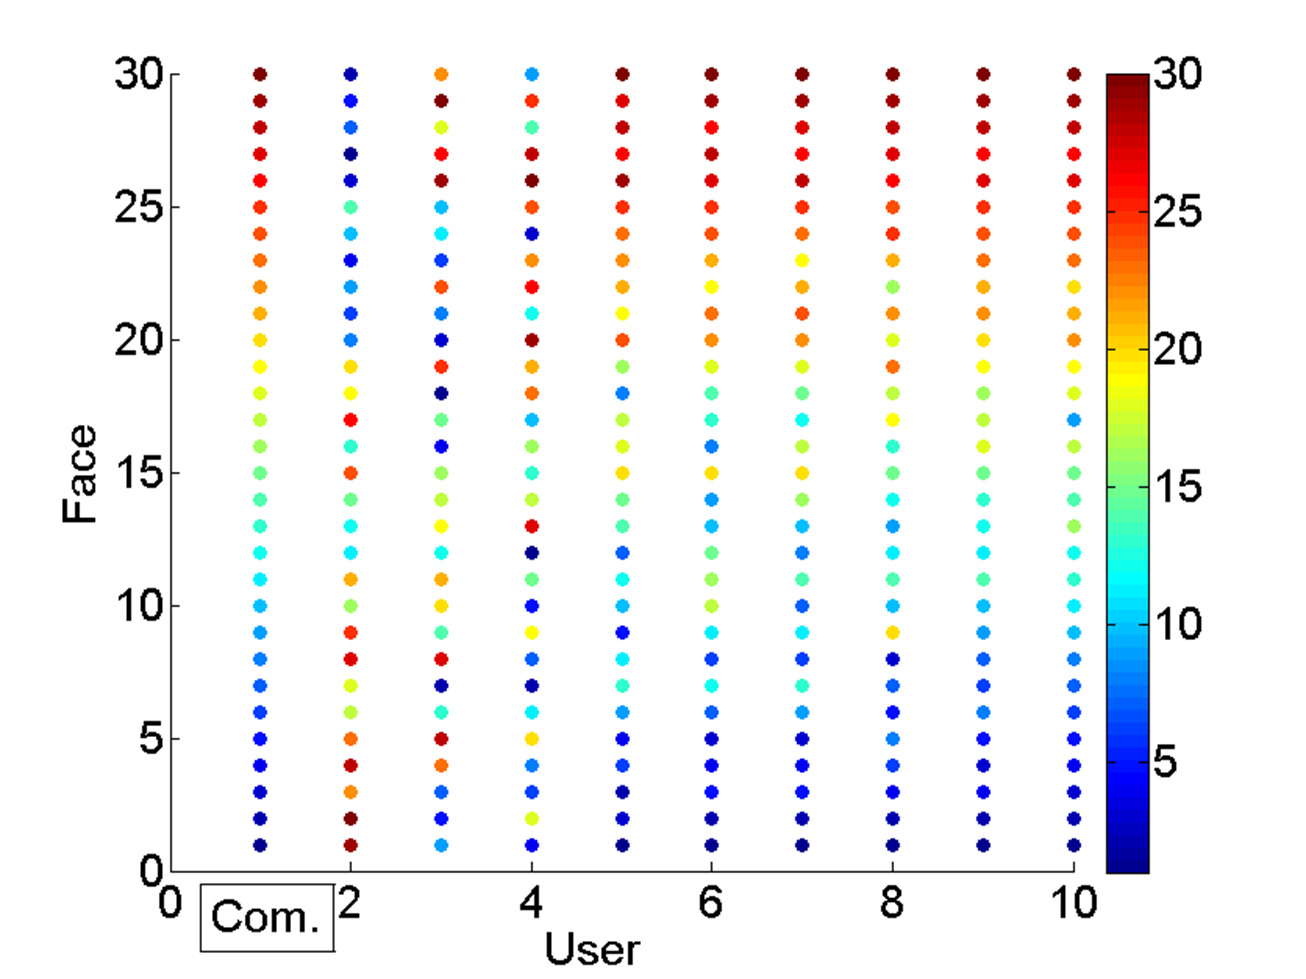
\includegraphics[width=0.3\textwidth]{age_position_color.png}}
   \subfigure[Bradley-Terry]{
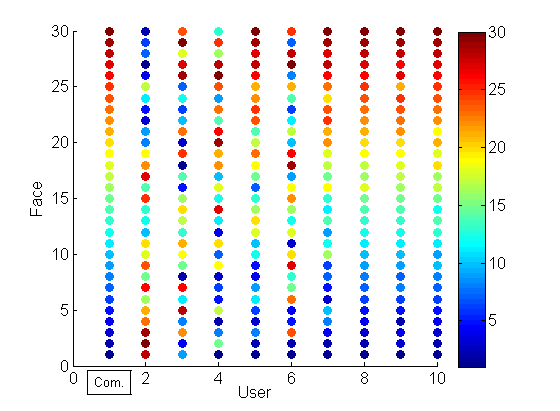
\includegraphics[width=0.3\textwidth]{model1_dot.png}}
\subfigure[Thurstone-Mosteller]{
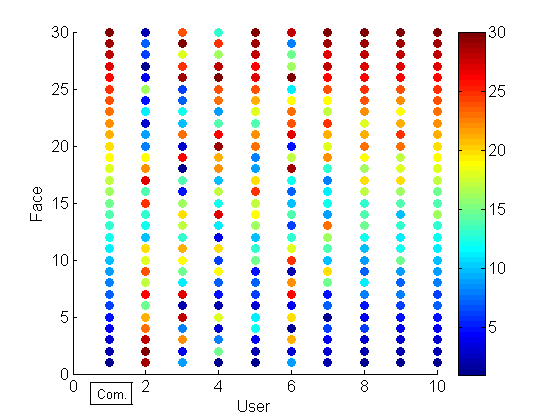
\includegraphics[width=0.3\textwidth]{model2_dot.png}}
  \caption{Comparison of common vs. personalized rankings of 9 representative annotators in Human age dataset.} \label{age_position_color}
\end{center}
\end{figure*}


\begin{figure*}
% \renewcommand{\captionfont}{\scriptsize \bfseries}
 \begin{center}
  \subfigure[L2 Loss]{
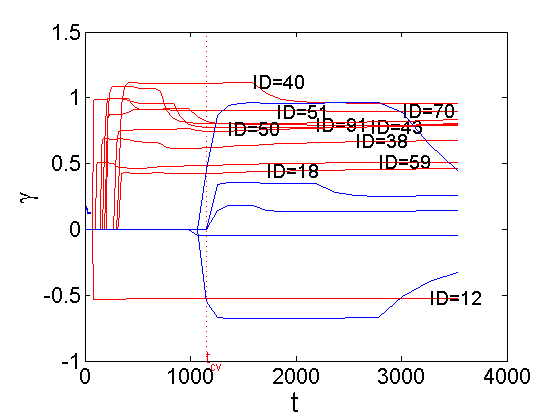
\includegraphics[width=0.3\textwidth]{L2-position-age.png}}
   \subfigure[Bradley-Terry]{
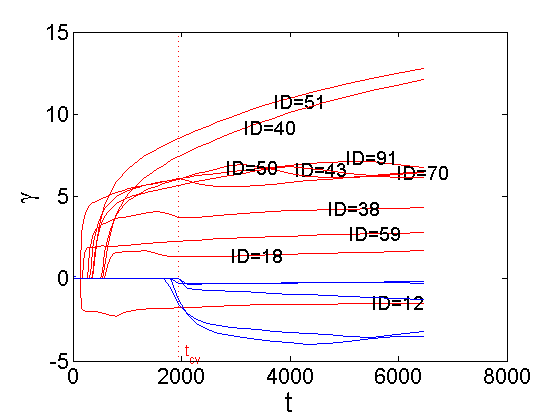
\includegraphics[width=0.3\textwidth]{model1-position-age.png}}
\subfigure[Thurstone-Mosteller]{
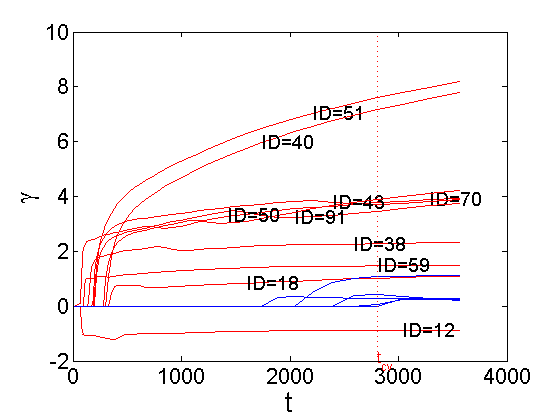
\includegraphics[width=0.3\textwidth]{model2-position-age.png}}
  \caption{LBI regularization path of $\gamma$ in Human age dataset. (Red: top 10 position-biased annotators; Blue: bottom 5 position-biased annotators)}\label{fig:ageposition}
\end{center}
\end{figure*}



{\renewcommand\baselinestretch{1.2}\selectfont
\setlength{\belowcaptionskip}{3pt}
\begin{table}[h]\caption{\label{tab:ageposition} Top 10 position-biased annotators in Human age dataset, together with the click counts of each side (i.e., Left and Right).}
\tiny
\centering
\newsavebox{\tablebox}
\begin{lrbox}{\tablebox}
\begin{tabular}{||c|c|c|c||c|c|c|c||}
  \hline  \textbf{Order} &\textbf{ID}   &\textbf{Left}  &\textbf{Right} & \textbf{Order} & \textbf{ID}   &\textbf{Left}  &\textbf{Right} \\
 \hline
\hline    1 & \textbf{12}	&90	&270  & 6 & \textbf{91}	&79	&5\\
\hline   2 & \textbf{70}	&191	&9 & 7 & \textcolor{blue}{\textbf{51}}	&63	&0\\
\hline    3 & \textbf{59}	&213	&66 & 8 & \textbf{50}	&60	&3 \\
\hline    4 & \textbf{38}	&110 &15  & 9 &\textbf{18}	&74	&25 \\
\hline    5 & \textbf{43}   &79 & 1 & 10 & \textcolor{blue}{\textbf{40}}	&40	&0   \\

\hline
\end{tabular}
\medskip
\end{lrbox}
\scalebox{1}{\usebox{\tablebox}}
\end{table}
\par}


\textbf{Settings} In this dataset, 30 images from human age dataset FG-NET \footnote{http://www.fgnet.rsunit.com/} are annotated by a group of volunteer users on \href{http://www.chinacrowds.com/}{ChinaCrowds} platform, as is illustrated in Fig.\ref{agedataset}. The annotator is presented with two images and
given a binary choice of which one is older. Totally, we obtain 14,011 pairwise comparisons from 94 annotators.

\textbf{Results} Tab.\ref{tab:age} shows the mean test error (70\% data for training, 30\% for testing)
results of 20 times achieved by this scheme. It is shown that consistent with the simulated data, in this dataset, the mixed-effects model with three losses could also provide
better approximate results of the annotators' preference than the HodgeRank estimator.\\

To further investigate the characteristics of annotators with personalized ranking, Fig.\ref{fig:agepreferencepath} illustrates annotator's LBI regularization paths of preference deviations with optimal $t$ (i.e., $t_{cv}$) returned by cross-validation in three losses. The red curves in Fig.\ref{fig:agepreferencepath} represent the top 10 annotators who jumped out early. It is easy to find that results returned by three losses are actually very similar except one or two differences. Besides, similar to the simulated data, annotators jumped out earlier are those with a large deviation ($L_2$-distance) from the common ranking and a big sample size showing high confidence of such deviations. Moreover, Fig.\ref{age_position_color} shows the order comparisons of common ranking (i.e., com.) and personalized ranking of 9 representative annotators at $t_{cv}$. The X-axis represents user index: user = 2, 3, 4 jumped out early corresponding to paths labeled with red stars in Fig.\ref{fig:agepreferencepath}; user = 5, 6, 7 jumped out in the middle time corresponding to green stars; user = 8, 9, 10 jumped out late corresponding to blue stars. The order of faces in Y-axis is arranged from lower to higher (i.e., from color blue to red) according to the common ranking score calculated by our method. The color represents the ranking position returned by the corresponding user. It is easy to see users jumped out late exhibit almost consistent ranking order with the common ranking, while the earlier ones are almost the adversarial against the common. A subset of this has been shown in Fig.\ref{fig:age0} in introduction.

Moreover, Fig.\ref{fig:ageposition} illustrates the LBI regularization paths of annotator's position bias with red lines represent the top 10 annotators. It is easy to see that the corresponding results returned from these three loss functions are exactly the same. Tab.\ref{tab:ageposition} further shows the click counts of each side (i.e., Left and Right) for these top 10 position-biased annotators.
It is easy to see that these annotators can be divided
into two types: (1) click one side all the time (with
ID in blue); (2) click one side with high probability
(others). Although it
might be relatively easy to identify the annotators of type (1) above
by inspecting their inputs, it is impossible for eye inspection
to pick up those annotators of type (2) with mixed rational and abnormal behaviors.
Therefore it is essential to design such a statistical methodology to
quantitatively detect these kind of position-biased annotators
for crowdsourcing platforms in market.



\begin{figure}[h]
%\setlength{\belowcaptionskip}{-22pt}
%\setlength{\abovecaptionskip}{5pt}
%\renewcommand{\captionfont}{\scriptsize \bfseries}
 \begin{center}
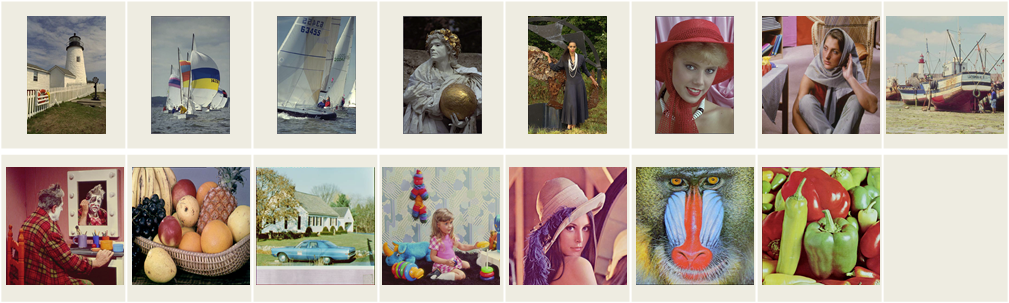
\includegraphics[width=0.8\linewidth]{iqa.png}
  \caption{Images in LIVE and IVC dataset.} \label{iqadataset}
\end{center}
\end{figure}



\subsection{Image Quality Assessment (IQA)}

\textbf{Settings} Two publicly available datasets, LIVE
\cite{LIVE} and IVC \cite{IVC}, are used in this work. The LIVE dataset contains 29 reference images and 779 distorted images. The distorted images are obtained using five different distortion processes--JPEG2000, JPEG, White Noise, Gaussian Blur, and Fast Fading Rayleigh. Considering the resolution limit of most test computers, we only choose 6 different reference images ($480 \times 720$) and 15 distorted versions of each reference, for a total of 96 images. The second dataset, IVC, which is also a broadly adopted dataset in the community of multimedia quality evaluation, includes 10 reference images and 185 distorted images derived from four distortion types--JPEG2000, JPEG, LAR Coding, and Blurring. Following the collection strategy in LIVE, we further select 9 different reference images ($512 \times 512$) and 15 distorted images of each reference. Totally, we obtain a medium-sized image set that contains a total of 240 images from 15 references, as illustrated in Fig.\ref{iqadataset}.
Finally, 342 observers of different
cultural background, each of whom performs a varied number of comparisons via Internet, provide
$52,043$  paired comparisons in total. The number of responses each reference image receives is different.



\begin{table}[t]\caption{\label{tab:iqa} HodgeRank vs. Mixed-effects model in IQA dataset (reference image 1).}
\centering
\begin{tabular}{lllll}
 \hline     &min  &mean &max &std\\
 \hline  HodgeRank     &0.1678    &0.1874    &0.2019    &0.0081 \\
\hline  L2 Loss     &0.1002    &\textcolor{red}{0.1094}    &0.1239    &0.0065  \\
\hline Bradley-Terry     &0.0638    &\textcolor{red}{0.0708}    &0.0817    &0.0054 \\
\hline Thurstone-Mosteller     &0.0625     &\textcolor{red}{0.0731}    &0.0825    &0.0057  \\
 \hline
 \end {tabular}
\end{table}




\begin{figure*}
% \renewcommand{\captionfont}{\scriptsize \bfseries}
 \begin{center}
  \subfigure[L2 Loss]{
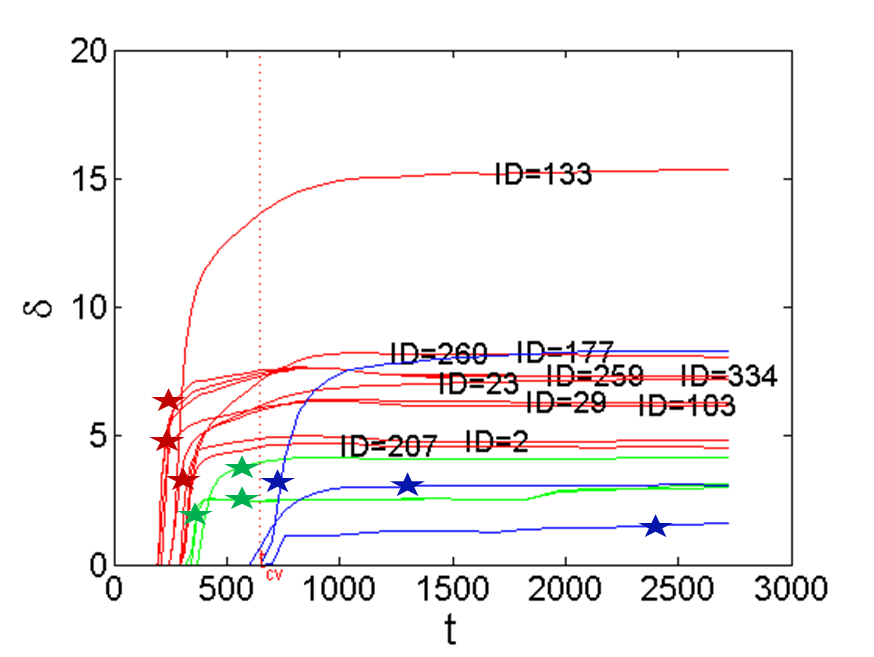
\includegraphics[width=0.3\textwidth]{iqa_l2_preference.png}}
   \subfigure[Bradley-Terry]{
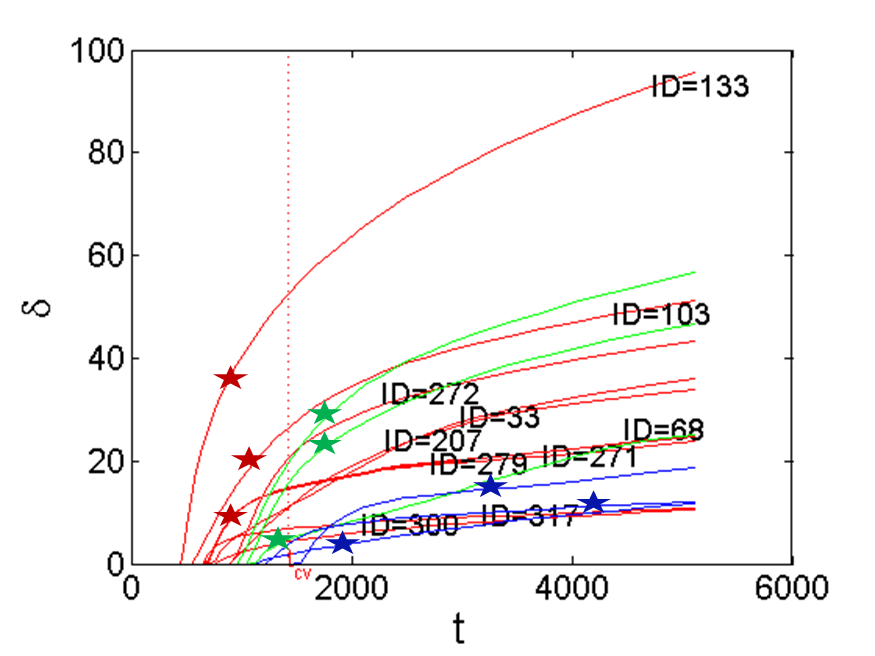
\includegraphics[width=0.3\textwidth]{iqa_model1_preference.png}}
\subfigure[Thurstone-Mosteller]{
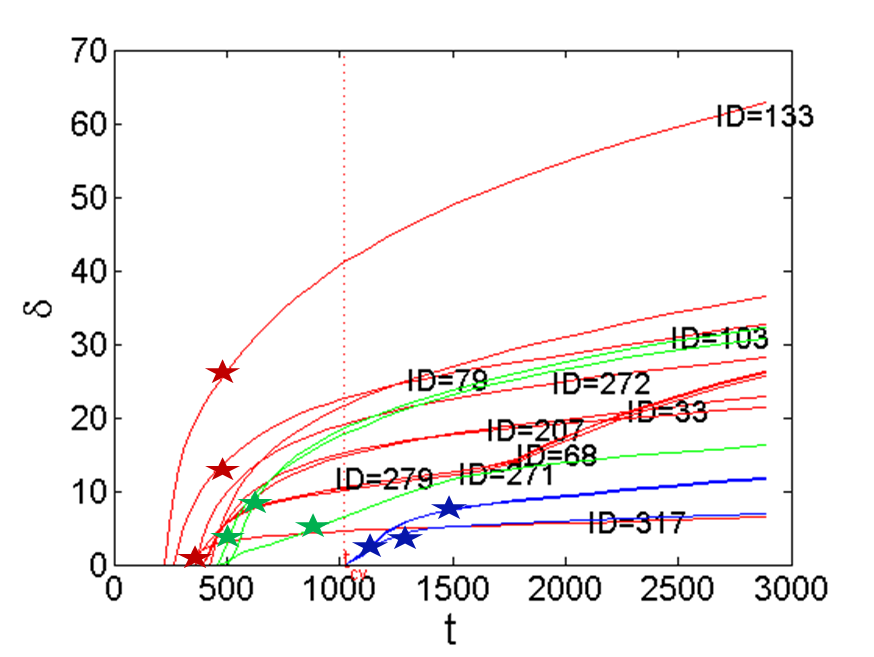
\includegraphics[width=0.3\textwidth]{iqa_model2_preference.png}}
  \caption{Top 10 annotators exhibiting personalized ranking in IQA dataset (reference image 1).}\label{fig:iqaref1preferencepath}
\end{center}
\end{figure*}




\begin{figure*}
% \renewcommand{\captionfont}{\scriptsize \bfseries}
 \begin{center}
  \subfigure[L2 Loss]{
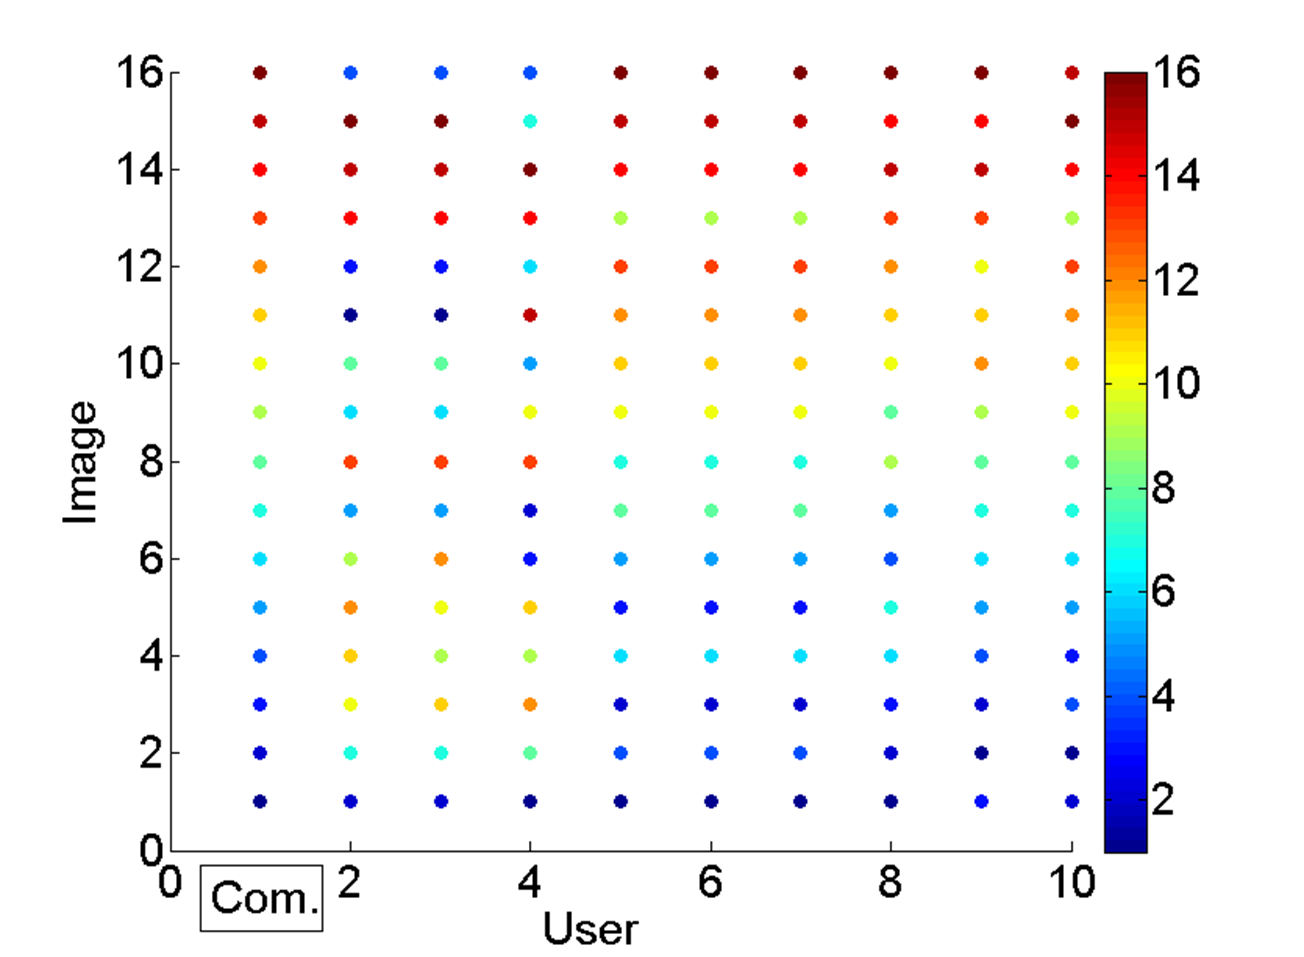
\includegraphics[width=0.3\textwidth]{iqa_position_color.png}}
   \subfigure[Bradley-Terry]{
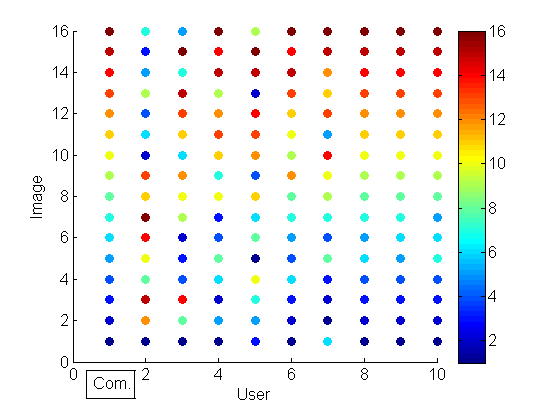
\includegraphics[width=0.3\textwidth]{iqa_dot_model1.png}}
\subfigure[Thurstone-Mosteller]{
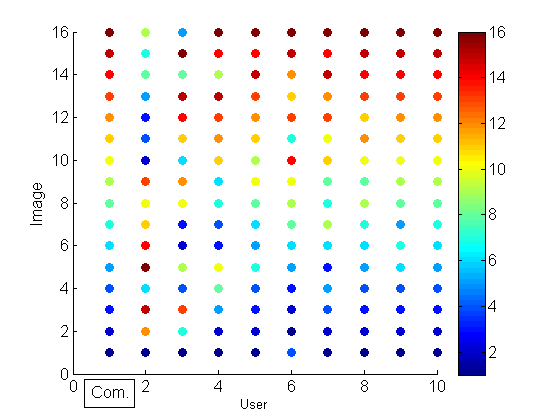
\includegraphics[width=0.3\textwidth]{iqa_dot_model2.png}}
  \caption{Comparison of common vs. personalized rankings of 9 representative annotators in IQA dataset (reference image 1).}  \label{iqa_position_color}
\end{center}
\end{figure*}


\begin{figure*}
% \renewcommand{\captionfont}{\scriptsize \bfseries}
 \begin{center}
  \subfigure[L2 Loss]{
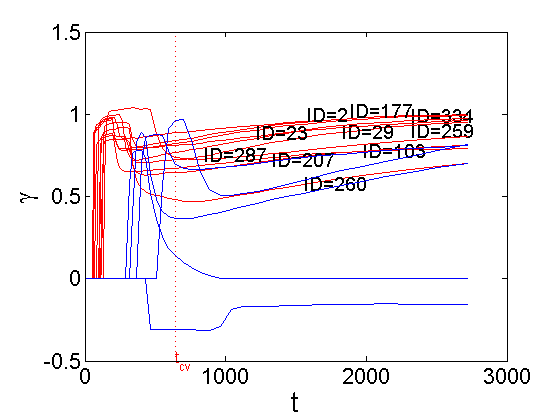
\includegraphics[width=0.3\textwidth]{iqa_l2_position.png}}
   \subfigure[Bradley-Terry]{
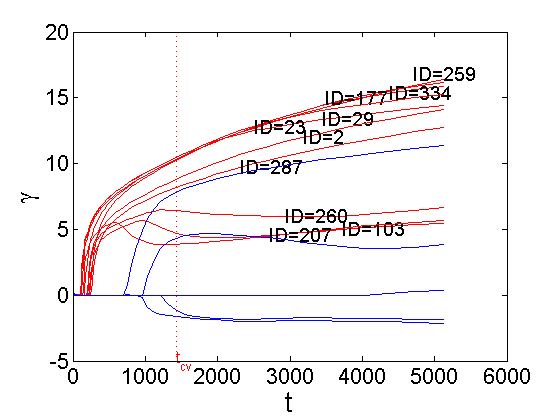
\includegraphics[width=0.3\textwidth]{iqa_model1_position.png}}
\subfigure[Thurstone-Mosteller]{
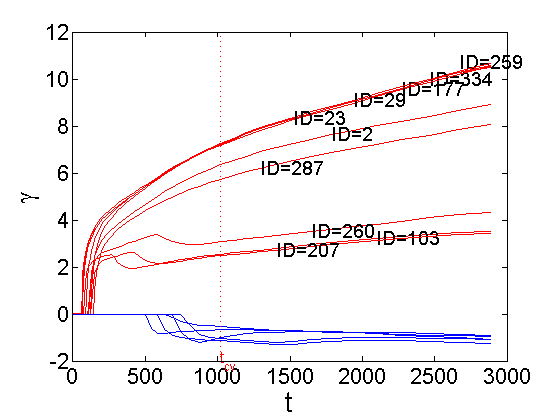
\includegraphics[width=0.3\textwidth]{iqa_model2_position.png}}
  \caption{LBI regularization path of $\gamma$ in IQA dataset (reference image 1). (Red: top 10 position-biased annotators; Blue: bottom 5 position-biased annotators).} \label{fig:iqa_position}
\end{center}
\end{figure*}

%%%%%%%%%%%%%%%%%%%%%%%%%%%%%%%%%%%%%%%%%%%%%%%%%%%%%%%%%%%%%%%%%%%%%%%%%%%%%








{\renewcommand\baselinestretch{1.1}\selectfont
\setlength{\belowcaptionskip}{0pt}
\begin{table}[h]\caption{\label{tab:ref1} Top 10 position-biased annotators in IQA dataset (reference image 1).}
\tiny
\centering
\begin{lrbox}{\tablebox}
\begin{tabular}{||c|c|c|c||c|c|c|c||}
  \hline  \textbf{Order} &\textbf{ID}   &\textbf{Left}  &\textbf{Right} & \textbf{Order} & \textbf{ID}   &\textbf{Left}  &\textbf{Right} \\
 \hline
 \hline  1 & \textcolor{blue}{\textbf{259}}    &96     &0  & 6 & \textcolor{blue}{\textbf{2}}   &55     &0 \\
\hline  2 & \textcolor{blue}{\textbf{334}}     &90    & 0  & 7 & \textbf{260}    & 49     &2\\
 \hline  3 & \textcolor{blue}{\textbf{177}}   &77     &0   & 8 & \textcolor{blue}{\textbf{23}}    &42     &0 \\
 \hline 4 & \textbf{103}  &74     &4  &9  & \textbf{207}    &46     &2\\
 \hline 5 & \textcolor{blue}{\textbf{29}}  &58     &0  & 10 & \textcolor{blue}{\textbf{287}}   &34     &0\\



 \hline
\end {tabular}
\medskip
\end{lrbox}
\scalebox{1}{\usebox{\tablebox}}
\end{table}
\par}

\begin{figure}[h]
%\setlength{\belowcaptionskip}{-22pt}
%\setlength{\abovecaptionskip}{5pt}
%\renewcommand{\captionfont}{\scriptsize \bfseries}
 \begin{center}
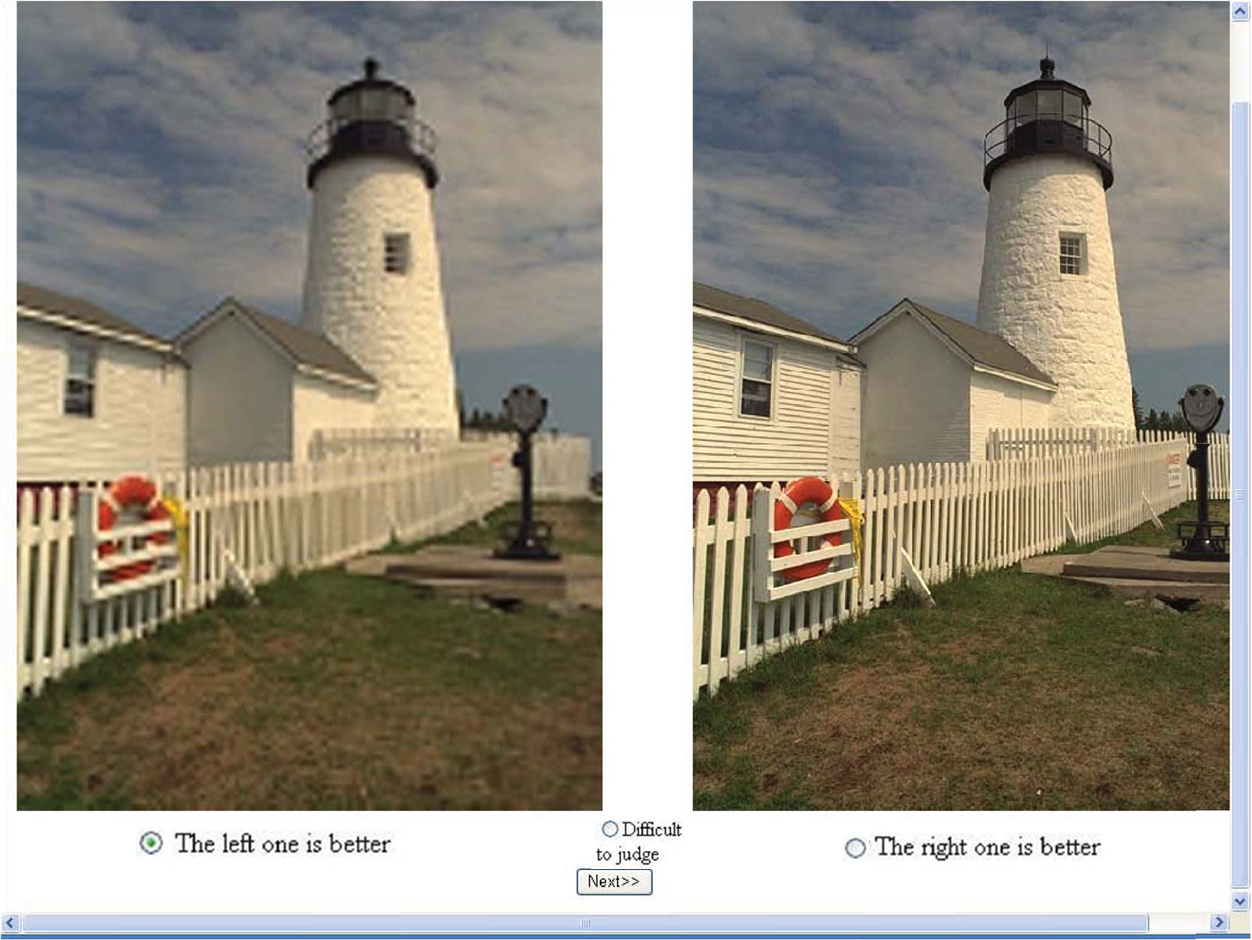
\includegraphics[width=0.7\linewidth]{iqa_test.png}
  \caption{Image quality assessment interface.} \label{iqa_test}
\end{center}
\end{figure}

To validate whether the annotators' preference function we estimated is good enough, we randomly take
reference image 1 as an illustrative example while other reference
images exhibit similar results.

\textbf{Results} In terms of prediction performance, it can be seen that the mixed-effects model with three losses is more accurate than HodgeRank by significantly reducing the mean test error, as is shown in Tab.\ref{tab:iqa}.

Besides, Fig.\ref{fig:iqaref1preferencepath} shows the regularization paths of personalized ranking with top 10 annotators (red curves) selected early in the paths.
Similar to the Age dataset, the common ranking vs. personalized ranking results of 9 representative users is shown in Fig.\ref{iqa_position_color}, corresponding to the red/green/blue stars in Fig.\ref{fig:iqaref1preferencepath}. \textcolor{red}{Note: Here, these exists large difference among the results returned by three losses, and we need more elegant words the explain this phenomenon............It is easy to see
that among the 10 annotators returned by L2 loss, 9 of them (except annotator
with ID = 133) click one side all the time (i.e., position-biased
annotators), while results returned by other two are not. From this viewpoint, maybe L2 loss is indeed less suitable for binary data on some specific cases compared with other two. Or, should we explain this phenomenon from a totally new perspective? add a remark here? }


Moreover, the LBI regularization paths of position bias $\gamma$ and click counts of top 10 annotators in this dataset are shown in Fig.\ref{fig:iqa_position} and Tab.\ref{tab:ref1}. It is easy to see that annotators picked out under three losses are also exactly the same, which are mainly those clicking on
one side almost all the time. Besides, it is interesting to see
that all these annotators highlighted with blue color in
Tab.\ref{tab:ref1} click the left side all the time. We then go back to
the crowdsourcing platform and find out that the reason behind
this is a \emph{default choice} on the left button, as is shown in Fig.\ref{iqa_test}, which induces
some lazy annotators to cheat for the task.



\subsection{WorldCollege Ranking}

\textbf{Settings} We now apply the proposed method to the WorldCollege dataset, which is composed of 261 colleges. Using the \href{http://www.allourideas.org/}{Allourideas} crowdsourcing platform, a total of 340 distinct annotators from various countries (e.g., USA, Canada, Spain, France, Japan)
are shown randomly with pairs of these colleges, and asked to decide which of the
two universities is more attractive to attend. Finally, we obtain a
total of 8,823 pairwise comparisons. The world map of all the annotators
is illustrated in Fig.\ref{map}.

\textbf{Results} We apply the proposed method to
the resulting dataset and find out that, similar to the simulation and other two real-world datasets, the mixed-effects model could produce better performance than Hodgerank with smaller mean test error, shown in Tab.\ref{tab:university}. Noting that in this dataset, only 9 annotators are treated as annotators with distinct personalized rankings at optimal $t$ (i.e., $t_{cv}$) selected via cross-validation in L2 loss case, as is shown in Fig.\ref{fig:univer_l2_preference}. The reason why others with relative big $\delta$ are not detected out lies in the small sample size they provide indicating high variances. To better illustrate comparison result of three losses, for other two, we also only pick up the top 9 annotators, as is shown in Fig.\ref{fig:univer_model1_preference} and \ref{fig:univer_model2_preference}. It is pleasing to see that the top 9 annotators returned by three losses are exactly the same in this dataset.
The common ranking vs. personalized ranking of 9 representative users is shown in Fig.\ref{university_position_color} with a similar observation to the other two datasets.
Besides, the regularization paths of position bias and click counts of top 10 annotators in this dataset are shown in Fig.\ref{fig:university_position} and Tab.\ref{tab:universityposition}.
It is easy to see that similar to the human age dataset, these annotators are either clicking one
side all the time, or clicking one side with high probability in mixed behaviors. Clearly, there is only one difference among these three cases, where L2 loss and Thurstone-Mosteller pick out annotator with ID=115, while Bradley-Terry treats annotator with ID=245 as position-biased one.
A further inspection of the dataset
confirms that such a detection result is reasonable, as the ratio of left/right clicks of these two annotators are 34:0 and 0:34 respectively, as is shown in Tab.\ref{tab:universityposition}.

\begin{figure}[h]
%\setlength{\belowcaptionskip}{-22pt}
%\setlength{\abovecaptionskip}{5pt}
%\renewcommand{\captionfont}{\scriptsize \bfseries}
 \begin{center}
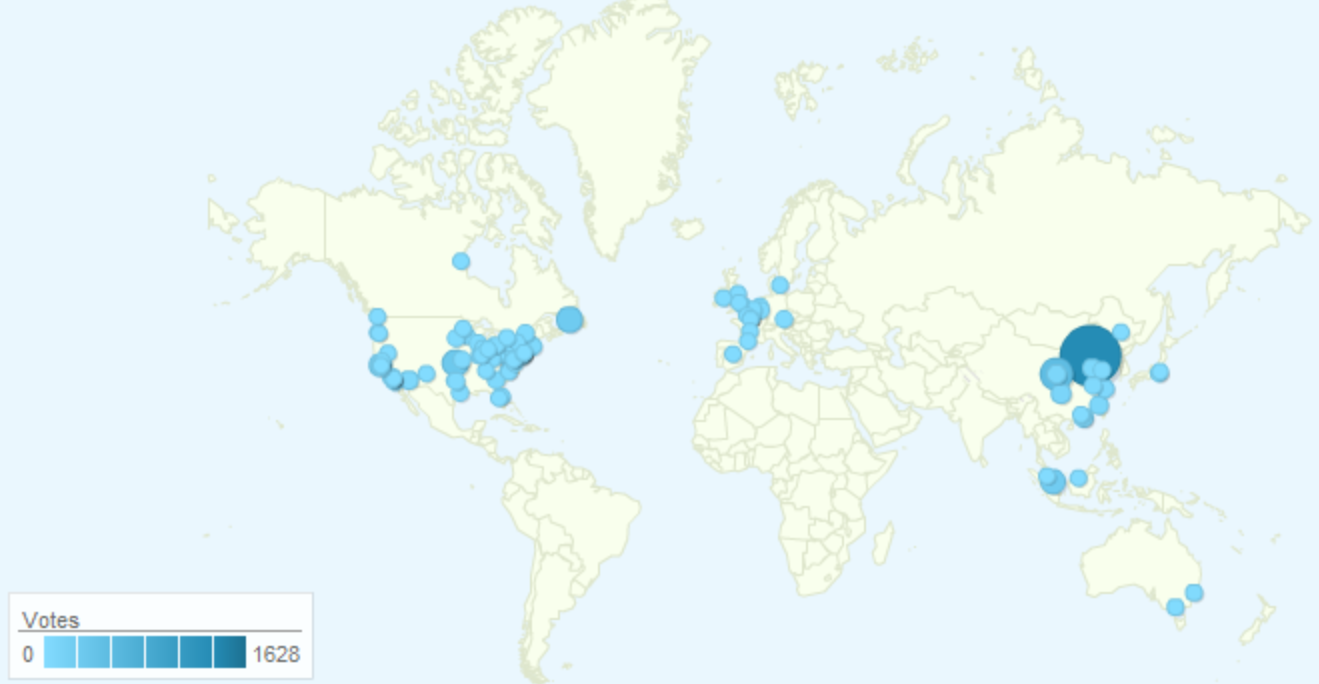
\includegraphics[width=0.55\linewidth]{map.png}
  \caption{World map of all the annotators in WorldCollege dataset.} \label{map}
\end{center}
\end{figure}

\begin{table}[h]\caption{\label{tab:university} HodgeRank vs. Mixed-effects model in WorldCollege ranking dataset.}
\centering
\begin{tabular}{lllll}
 \hline     &min  &mean &max &std\\
 \hline  HodgeRank     &0.2979    &0.3108    &0.3230    &0.0097  \\
\hline  L2 Loss      &0.2530    &\textcolor{red}{0.2670}    &0.2757    &0.0071  \\
\hline Bradley-Terry     &0.2456    &\textcolor{red}{0.2555}    &0.2678    &0.0099 \\
\hline Thurstone-Mosteller      &0.2553    &\textcolor{red}{0.2616}    &0.2696    &0.0067  \\
 \hline
 \end {tabular}
\end{table}




\begin{figure*}
% \renewcommand{\captionfont}{\scriptsize \bfseries}
 \begin{center}
  \subfigure[L2 Loss]{
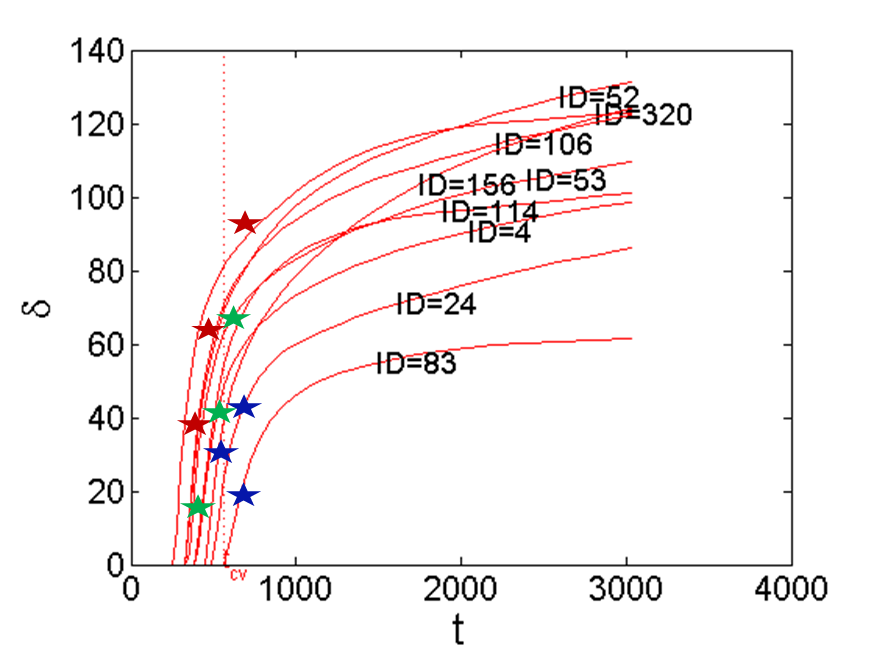
\includegraphics[width=0.3\textwidth]{univer_l2_preference.png}\label{fig:univer_l2_preference}}
   \subfigure[Bradley-Terry]{
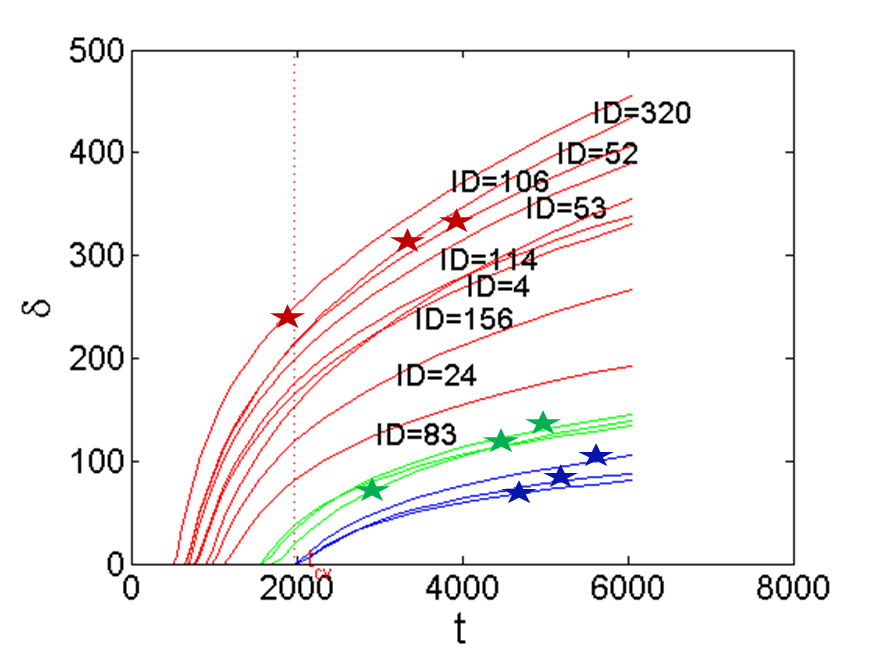
\includegraphics[width=0.3\textwidth]{univer_model1_preference3.png}\label{fig:univer_model1_preference}}
\subfigure[Thurstone-Mosteller]{
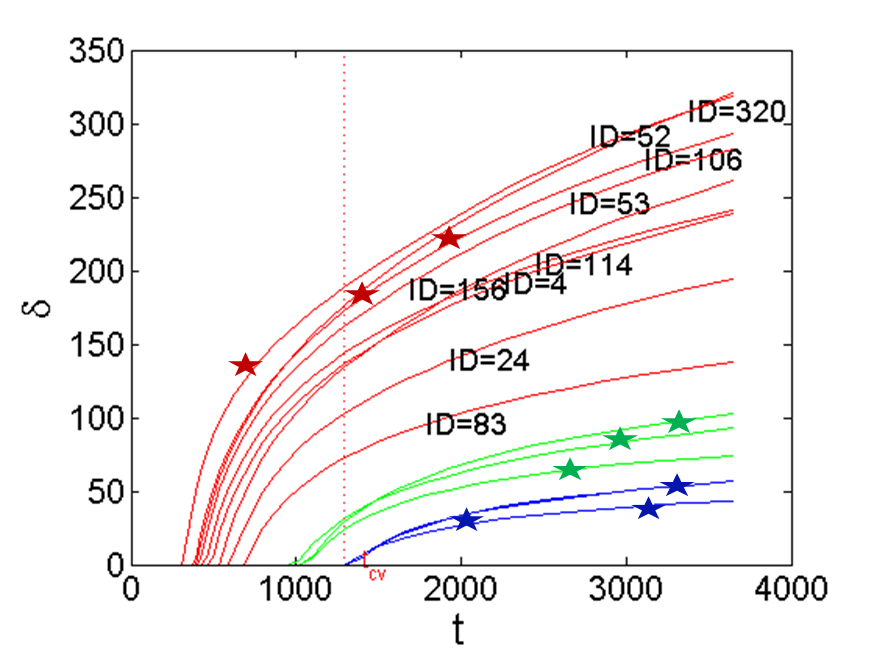
\includegraphics[width=0.3\textwidth]{univer_model2_preference3.png}\label{fig:univer_model2_preference}}
  \caption{Top 9 annotators exhibiting personalized ranking in WorldCollege ranking dataset.}
\end{center}
\end{figure*}






\begin{figure*}
% \renewcommand{\captionfont}{\scriptsize \bfseries}
 \begin{center}
  \subfigure[L2 Loss]{
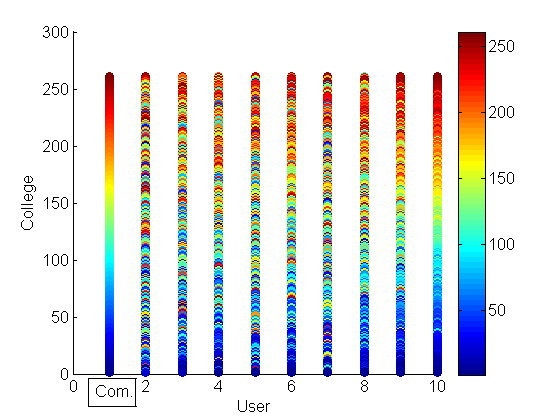
\includegraphics[width=0.3\textwidth]{univer_l2_dot_new.png}}
   \subfigure[Bradley-Terry]{
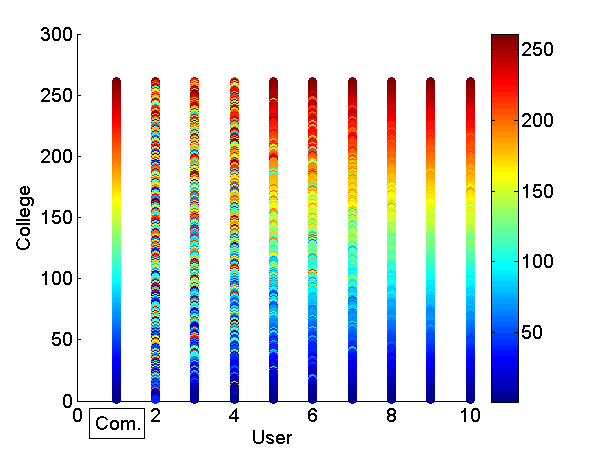
\includegraphics[width=0.3\textwidth]{univer_model1_dot3.png}}
\subfigure[Thurstone-Mosteller]{
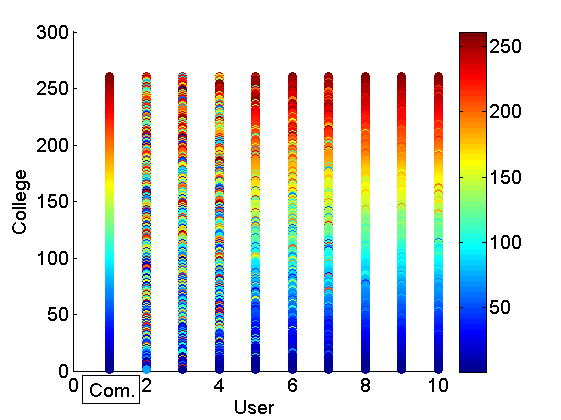
\includegraphics[width=0.3\textwidth]{univer_model2_dot3.png}}
 \caption{Comparison of common vs. personalized rankings of 9 annotators in WorldCollege ranking dataset.} \label{university_position_color}
\end{center}
\end{figure*}


%\begin{figure}[h]
%%\setlength{\belowcaptionskip}{-22pt}
%%\setlength{\abovecaptionskip}{5pt}
%%\renewcommand{\captionfont}{\scriptsize \bfseries}
% \begin{center}
%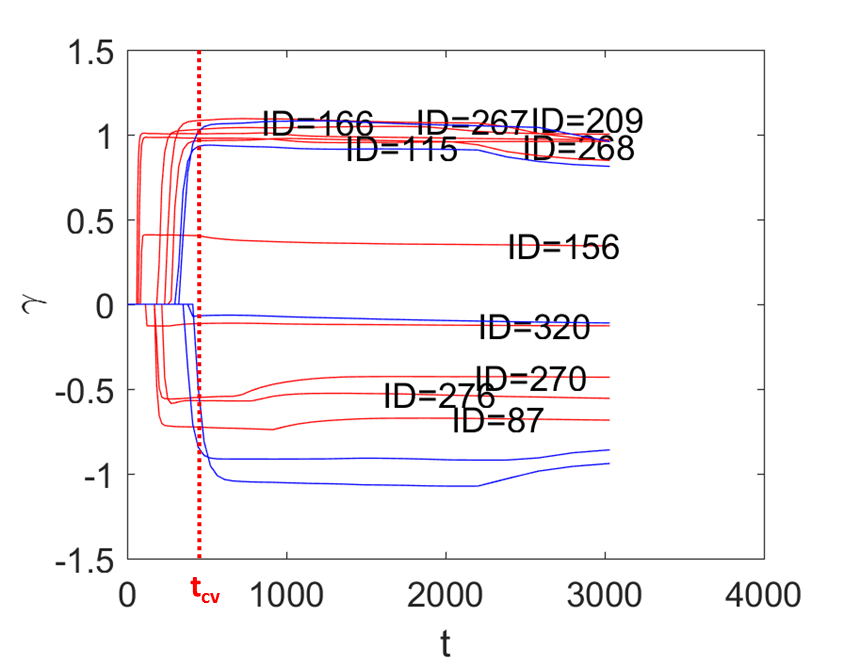
\includegraphics[width=0.7\linewidth]{university_position_optimal.png}
%  \caption{LBI regularization path of $\gamma$ in WorldCollege ranking dataset. (Red: top 10 position-biased annotators; Blue: bottom 5 position-biased annotators).} \label{fig:university_position}
%\end{center}
%\end{figure}


\begin{figure*}[htb]
% \renewcommand{\captionfont}{\scriptsize \bfseries}
 \begin{center}
  \subfigure[L2 Loss]{
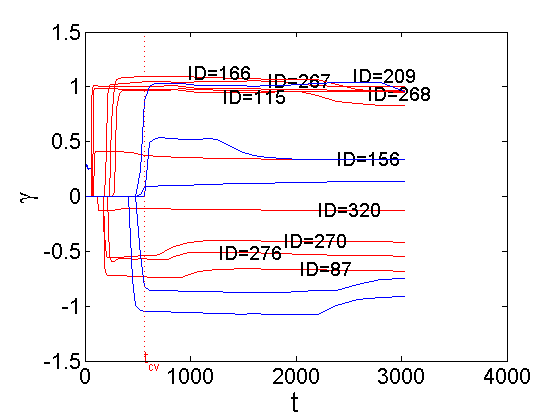
\includegraphics[width=0.3\textwidth]{univer_l2_position.png}}
   \subfigure[Bradley-Terry]{
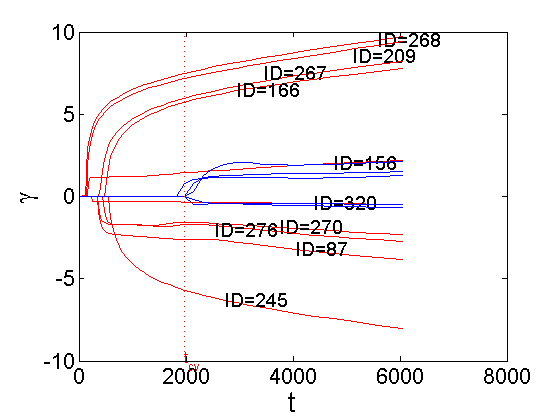
\includegraphics[width=0.3\textwidth]{univer_model1_position.png}}
\subfigure[Thurstone-Mosteller]{
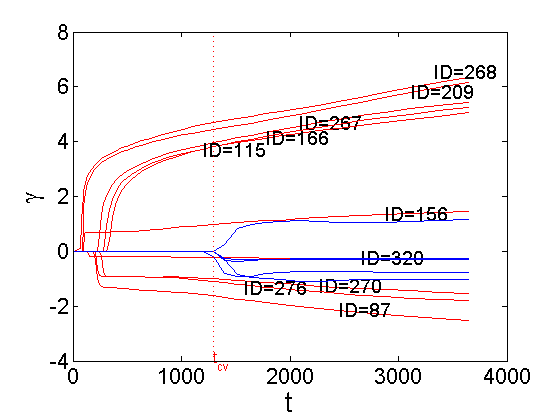
\includegraphics[width=0.3\textwidth]{univer_model2_position.png}}
  \caption{LBI regularization path of $\gamma$ in WorldCollege ranking dataset. (Red: top 10 position-biased annotators; Blue: bottom 5 position-biased annotators).} \label{fig:university_position}
\end{center}
\end{figure*}




{\renewcommand\baselinestretch{1.3}\selectfont
\setlength{\belowcaptionskip}{0pt}
\begin{table}[h]\caption{\label{tab:universityposition} Top 10 position-biased annotators in WorldCollege ranking dataset.}
\tiny
\centering
\begin{lrbox}{\tablebox}
\begin{tabular}{||c|c|c|c||c|c|c|c||}
  \hline  \textbf{Order} &\textbf{ID}   &\textbf{Left}  &\textbf{Right} & \textbf{Order} & \textbf{ID}   &\textbf{Left}  &\textbf{Right} \\
 \hline
 \hline  1 & \textcolor{blue}{\textbf{268}} &148	&0 & 6 & \textbf{270}	&20	&70 \\
 \hline  2 & \textcolor{blue}{\textbf{209}}	&127	&0 & 7 & \textcolor{blue}{\textbf{267}}	&45	&0 \\
 \hline 3 & \textbf{156}	&189	&67 & 8 & \textbf{276}	&16	&54 \\
 \hline 4  & \textbf{320}	&253	&324  & 9 & \textcolor{blue}{\textbf{166}}	&35	&0 \\
 \hline 5 & \textbf{87}	&11	&62 & 10 & \textcolor{blue}{\textbf{115}}	&34	&0 \\
 \hline   &  	& 	&  & 10 & \textcolor{blue}{\textbf{245}}	&0	&34 \\



 \hline
\end {tabular}
\medskip
\end{lrbox}
\scalebox{1}{\usebox{\tablebox}}
\end{table}
\par}


%\begin{figure}
%%\setlength{\belowcaptionskip}{-22pt}
%%\setlength{\abovecaptionskip}{5pt}
%%\renewcommand{\captionfont}{\scriptsize \bfseries}
% \begin{center}
%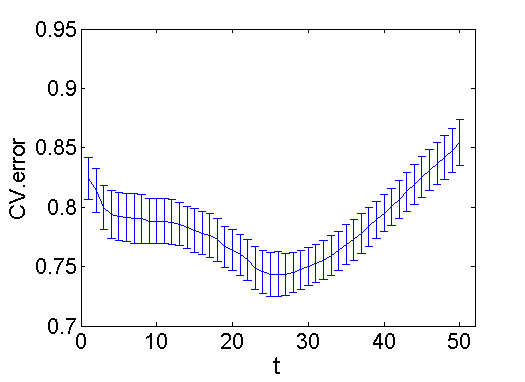
\includegraphics[width=\linewidth]{university.png}
%  \caption{university} \label{university}
%\end{center}
%\end{figure}








\section{Conclusions}\label{sec:conclusion}

In this paper, we propose a parsimonious mixed-effects model based on HodgeRank to learn user's preference or utility function in crowdsourced ranking, which
takes into account both the personalized preference deviations from the common and position biases of the annotators.
To be specific, common preference scores indicate the consistent ranking on population-level which approximates the behavior of
all users, while a small set of annotators might have nonzero
personalized deviations and abnormal behavior in position bias. Equipped with the newly developed Linearized
Bregman Iteration, which is a simple iterative procedure generating a sequence of parsimonious models,  we establish a dynamic path from the common utility to individual
variations, with different levels of parsimony or sparsity on personalization. In this dynamic scheme, three kinds of losses are systematically discussed, including  L2 loss, Bradley-Terry, Thurstone-Mosteller.
Experimental studies conducted on simulated examples and real-world
datasets show that our proposed method could exhibit better performance (i.e.
smaller test error) compared with HodgeRank. 
Our results suggest that the proposed methodology is an effective tool to investigate the diversity in annotator's behavior
in modern crowdsourcing data.

\ifCLASSOPTIONcaptionsoff
  \newpage
\fi


\bibliographystyle{abbrv}
 \bibliography{sigproc}

% if you will not have a photo at all:
\vspace{0cm}\begin{biography}[{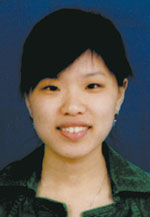
\includegraphics[width=1in,height=1.25in,clip,keepaspectratio]{qqxu}}]{Qianqian Xu received the B.S. degree in computer science from China University of Mining and Technology in 2007 and the Ph.D. degree in computer science from University of Chinese Academy of Sciences in 2013. She is currently an Associate Professor with the Institute of Information Engineering, Chinese Academy of Sciences, Beijing, China. Her research interests include statistical machine learning, with applications in multimedia and computer vision. She has authored or coauthored 10+ academic papers in prestigious international journals and conferences, among which she has published 4 full papers with the first author's identity in ACM Multimedia (acceptance rate 17\%).  She served as member of professional committee of CAAI, and member of online program committee of VALSE, etc.}
\end{biography}

\vspace{0cm}\begin{biography}[{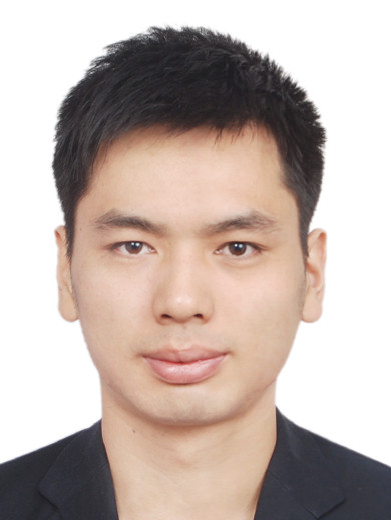
\includegraphics[width=1in,height=1.25in,clip,keepaspectratio]{jcxiong}}]{Jiechao Xiong is currently pursuing the Ph.D. degree in statistics at the School of Mathematical Science, Peking University, Beijing, China. His research interests include statistical learning, data science and topological and geometric methods for high-dimension data analysis.}
\end{biography}

\vspace{0cm}\begin{biography}[{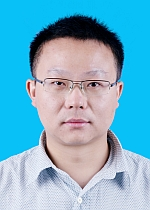
\includegraphics[width=1in,height=1.25in,clip,keepaspectratio]{xccao}}]{Xiaochun Cao, Professor of the Institute of Information Engineering, Chinese Academy of Sciences. He received the B.E. and M.E. degrees both in computer science from Beihang University (BUAA), China, and the Ph.D. degree in computer science from the University of Central Florida, USA, with his dissertation nominated for the university level Outstanding Dissertation Award. After graduation, he spent about three years at ObjectVideo Inc. as a Research Scientist. From 2008 to 2012, he was a professor at Tianjin University. He has authored and coauthored over 100 journal and conference papers. In 2004 and 2010, he was the recipients of the Piero Zamperoni best student paper award at the International Conference on Pattern Recognition. He is a fellow of IET and a Senior Member of IEEE. He is an associate editor of IEEE Transactions on Image Processing.}
\end{biography}

\vspace{0cm}\begin{biography}[{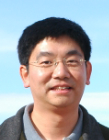
\includegraphics[width=1in,height=1.25in,clip,keepaspectratio]{yuany}}]{Yuan Yao received the B.S.E and M.S.E in control engineering both from Harbin Institute of Technology, China, in 1996 and 1998, respectively,
M.Phil in mathematics from City University of Hong Kong in 2002, and Ph.D. in mathematics from the University of California, Berkeley, in 2006. Since then he has been with Stanford University and in 2009, he joined the School of Mathematical Sciences, Peking University, Beijing, China, as a professor of statistics in the Hundred Talents Program. His current research interests include topological and geometric methods for high dimensional data analysis and statistical machine learning, with applications in computational biology, computer vision, and information retrieval. Dr. Yao is a member of American Mathematical Society (AMS), Association for Computing Machinery (ACM), Institute of Mathematical Statistics (IMS), and Society for Industrial and Applied Mathematics (SIAM). He served as area or session chair in NIPS and ICIAM, as well as a reviewer of Foundation of Computational Mathematics, IEEE Trans. Infomation Theory, J.  Machine Learning Research, and Neural Computation, etc.}
\end{biography}
%


% insert where needed to balance the two columns on the last page pwith
% biographies
%\newpage


% You can push biographies down or up by placing
% a \vfill before or after them. The appropriate
% use of \vfill depends on what kind of text is
% on the last page and whether or not the columns
% are being equalized.

%\vfill

% Can be used to pull up biographies so that the bottom of the last one
% is flush with the other column.
%\enlargethispage{-5in}


%%\section{Proofs}
%\begin{proof}[Proof of Theorem \ref{thm:LASSO}]
%The theorem mainly follows the Theorem 1 in \cite{Wainwright09} by changing the notation from $X,\beta,n,p,\gamma,\lambda_n$ to $\Psi,\gamma,l,m,\eta,\lambda/l$. Note that in \cite{Wainwright09}, column normalization $\mu_\Psi=1$ is assumed, while in this paper we keep this parameter $\mu_\Psi\le 1$. Our results here assume Gaussian noise, which can be extended to sub-Gaussian noise in \cite{Wainwright09} resulting to a slight different $\lambda$ up to a constant $\sqrt{2}$ as well as a different constant in $l_\infty$ bound. %is due to the assumption of noise, gaussian or sub-gaussian. The main difference is the . Here we do more careful calculation on bounding the tail probability of gaussian noise. %\textcolor[rgb]{1.00,0.00,0.00}{(Actually the constant in \cite{Wainwright09} is somewhat wrong.)}
%\end{proof}
%
%\begin{proof}[Proof of Theorem \ref{thm:LB}] Here we present a self-contained sketchy proof, leaving the readers to \cite{osher2014} for a full development of the related theory.
%
%\textbf{(No-false-positive)} First consider the LBI restricted on $S$
%\begin{equation}\label{eq:psub}
%(p_S^{k+1} + \gamma_S^{k+1}/\kappa) - (p_S^k + \gamma_S^k/\kappa) = \Psi^T_S\Psi_S(\tilde{\gamma}_S - \gamma_S^k)\triangle t
%\end{equation}
%where $\tilde{\gamma}_S = \gamma_S^\ast+ (\Psi^T_S\Psi_S)^{-1}\Psi^T_S\Psi\epsilon$. %Note that the update of $\gamma^k_S$ is actually gradient decent on the active set with step size $h = \kappa\triangle t$.
%
%Note that $\|\Psi_S(\tilde{\gamma}_S - \gamma^k)\|$ is monotonically decreasing under the condition $h\|\Psi^T_S\Psi_S\|<2$. In fact,
%\begin{eqnarray}\nonumber
%&&\|\Psi_S(\tilde{\gamma}_S - \gamma^{k+1})\|^2 - \|\Psi_S(\tilde{\gamma}_S - \gamma^k)\|^2 \\\nonumber
%&=& \|\Psi_S(\gamma^{k+1}-\gamma^k)\|^2 + 2(\gamma^{k+1}-\gamma^k)^T\Psi_S^T\Psi_S(\gamma^{k}-\tilde{\gamma}_S)\\\nonumber
%&=& \|\Psi_S(\gamma^{k+1}-\gamma^k)\|^2 - 2/\triangle t (\gamma^{k+1}-\gamma^k)^T  \ldots \\\nonumber
% &&\cdot [(p_S^{k+1} - p_S^k)+ (\gamma_S^{k+1}/\kappa - \gamma_S^k/\kappa)]  \\\nonumber
% &\le&\|\Psi_S(\gamma^{k+1}-\gamma^k)\|^2 \ldots \\\nonumber
%  &&- 2/\triangle t (\gamma^{k+1}-\gamma^k)^T (\gamma_S^{k+1}/\kappa - \gamma_S^k/\kappa)     \\\nonumber
% &=& (\gamma^{k+1}-\gamma^k)^T (\Psi_S^T\Psi_S-2/h) (\gamma^{k+1}-\gamma^k) \\\nonumber
% &\le& 0,
%\end{eqnarray}
%where we have used $(\gamma^{k+1}-\gamma^k)^T ((p_S^{k+1} - p_S^k)\ge 0$ since $\gamma_i (p_i - p^\prime_i) = |\gamma_i| - \gamma_i p_i^\prime \geq 0$.
%Using this fact, we can roughly see $\gamma^k_S$ is bounded. Actually,
%\begin{eqnarray*}
%\|\gamma^k_S\|_\infty &\le& \|\tilde{\gamma}_S\|_\infty + \|\tilde{\gamma}_S - \gamma^k_S\|_2\\ \nonumber
% &\le& \|\tilde{\gamma}_S\|_\infty  + \frac{\|\Psi_S(\tilde{\gamma}_S - \gamma^k_S)\|_2}{\sqrt{lC_{min}}} \\
% &\le& \|\tilde{\gamma}_S\|_\infty  + \frac{\|\Psi_S(\tilde{\gamma}_S - \gamma^0_S)\|_2}{\sqrt{lC_{min}}}.
% \end{eqnarray*}
% Using concentration inequality, we can bound the last term by $B$ with high probability (at least $1-1/(m \sqrt{\log m})-1/(n\sqrt{\log n})$ via a Gaussian tail bound).
%
% Now we turn to the LBI restricted on $T = S^c$ with $\gamma^k_S$ above.
% \begin{eqnarray*}
%&&(p_{T}^{k+1} + \gamma_T^{k+1}/\kappa) - (p_T^k + \gamma_T^k/\kappa) \\\nonumber
%&= &\Psi^T_T\Psi_S(\gamma_S^\ast - \gamma_S^k)\triangle t + \Psi^T_T\Psi\epsilon \\\nonumber
%&=& \Psi^T_T\Psi_S^\dagger[(p_S^{k+1} - p_S^k)+ (\gamma_S^{k+1}/\kappa - \gamma_S^k/\kappa)] + \Psi^T_TP_T\Psi\epsilon
%\end{eqnarray*}
%where $P_T = I-P_S = I - \Psi_S^\dagger \Psi_S^T$ is the projection matrix onto $\im(\Psi_T)$.
%
%A telescope sum on both sides with $p^0=\gamma^0=0$,
%\[ p^k_T + \gamma^k_T/\kappa= \Psi^\ast_{T} \Psi_S^\dagger  (p^k_S + \gamma^k_S/\kappa) + t_k \Psi^\ast_T P_{T} \Psi\epsilon.\]
%
%Now consider the $l_\infty$-norm of the right side. If it is smaller than 1, then $\gamma^k_T = 0$ which implies no-false-positive. Note that the first part
%\begin{eqnarray*}
%\| \Psi^\ast_{T} \Psi_S^\dagger  (p^k_S+\gamma^k_S/\kappa)\|_\infty & \leq & (1-\eta)(1+ \|\gamma^k_S\|_\infty/\kappa)  \\
%&\leq & 1 - (1 - B/\kappa\eta)\eta
%\end{eqnarray*}
%Also we have $\|\Psi^T_TP_T\Psi\epsilon\|\le 2\sigma\mu_\Psi\sqrt{\log m/l}$ with high probability (at least $1-1/(m \sqrt{\log m})$ via a Gaussian tail bound), so when $t^k\le \bar{\tau}$, the second term is smaller than $(1 - B/\kappa\eta)\eta$. Hence the whole term is less than 1, as desired.
%
%\textbf{(Sign-consistency)} Given no-false-positive before $\bar{\tau}$, to achieve sign consistency, we only need to show \eqref{eq:psub} can achieve no-false-negtive before $\bar{\tau}$.
%
%Denote $\Phi_k= |\tilde{\gamma}_S| - |\gamma^k_S| - <p^k_S, \tilde{\gamma}_S - \gamma^k_S> + \frac{||\tilde{\gamma}_S - \gamma^k_S||^2}{2\kappa}$ and
%\begin{equation} \label{eq:F}
%F(x) = \frac{x}{2\kappa}+ \begin{cases} 0 & 0 \leq x < \tilde{\gamma}^{2}_{min} \\
%2x/\tilde{\gamma}_{min} & \tilde{\gamma}_{min}^{2} \leq x \leq s\tilde{\gamma}_{min}^{2} \\
%2\sqrt{xs} & x \geq s\tilde{\gamma}_{min}^{2}
%\end{cases}
%\end{equation}
%which is monotonically nondecreasing and right continuous.
%Then $F(||\tilde{\gamma}_S - \gamma^k_S||^2)\ge\Phi_k$, or equivalently $||\tilde{\gamma}_S - \gamma^k_S||^2\ge F^{-1}(\Phi_k)$, where $F^{-1}$ is the right-continuous inverse of $F$.
%
%Next we are going to show $\Phi_k$ is decreasing at least
%\begin{equation} \label{eq:phidrop}
%\Phi_{k+1} - \Phi_{k} \leq -\triangle t \tilde{C}_{min} F^{-1}(\Psi_k) .
%\end{equation}
%where $\tilde{C}_{min} = C_{min} l (1-h\|\Psi_S\Psi_S^T\|/2)$. With a sufficient fast drop of $\Phi_k$, we just need to show $\Phi_k \le \tilde{\gamma}_{min}^2/(2\kappa)$, which is sufficient for no-false-negative, i.e., every outlier in $S$ has been found by $\gamma_k$.
%
%Multiplying $\tilde{\gamma}_S - \gamma^k_S$ on the both sides of \eqref{eq:psub}, gives
% \begin{eqnarray*}
%&&\Phi_{k+1} - \Phi_k + (p_S^{k+1}-p_S^k)\gamma^k_S -\|\gamma^{k+1}_S - \gamma^k_S\|^2/2\kappa \\\nonumber
% &=& -\triangle t\left<\tilde{\gamma}_S - \gamma^k_S,\Psi^T_S\Psi_S(\tilde{\gamma}_S - \gamma^k_S) \right>
% \end{eqnarray*}
%Since for $i \in S$, $(p_i^{k+1}-p_i^k)\gamma^{k+1}_{i} = |\gamma^{k+1}_{i} | - p_i^k\gamma^{k+1}_{i}\ge 0$,
%%and $(p^{(i)}_{k+1}-p^{(i)}_k)(u^{(i)}_{k+1}-u^{(i)}_{k}) \ge 0$, \\
%\begin{eqnarray}\nonumber
%&&\|\gamma^{k+1}_S - \gamma^k_S\|^2/\kappa - 2(p_S^{k+1}-p_S^k)\gamma^k_S \\\nonumber
%&\le& \|\gamma^{k+1}_S - \gamma^k_S\|^2/\kappa + 2(p_S^{k+1}-p_S^k)(\gamma^{k+1}_S-\gamma^k_S)\\\nonumber
%&\le& \|\gamma^{k+1}_S - \gamma^k_S\|^2/\kappa + 2(p_S^{k+1}-p_S^k)(\gamma^{k+1}_S-\gamma^k_S)\\\nonumber
%    && +\kappa\|p_S^{k+1}-p_S^k\|^2\\ \nonumber
% &\le& \kappa\| p_S^{k+1}-p_S^k + (\gamma^{k+1}_S - \gamma^k_S)/\kappa\|^2 \\ \nonumber
% &=& \kappa \triangle t^2\| \Psi^T_S\Psi_S(\tilde{\gamma}_S - \gamma^k_S)\|^2 \nonumber
%\end{eqnarray}
%So for $h=\kappa \triangle t$,
%\begin{eqnarray}\nonumber
%&&\Phi_{k+1} - \Phi_k \\ \nonumber
%&\le& -\triangle t \left<\Psi_S (\tilde{\gamma}_S - \gamma^k_S),\Psi_S (\tilde{\gamma}_S - \gamma^k_S) \right> \\ \nonumber
% &&+ \frac{ \kappa  \triangle t^2}{2} \left<\Psi^T_S\Psi_S(\tilde{\gamma}_S - \gamma^k_S),\Psi^T_S\Psi_S(\tilde{\gamma}_S - \gamma^k_S)\right>\\ \nonumber
%&=& -\triangle t \left<\Psi_S(\tilde{\gamma}_S - \gamma^k_S), (I - h \Psi^T_S\Psi_S/2) \Psi_S(\tilde{\gamma}_S - \gamma^k_S) \right>\\ \nonumber
%&\le& -\triangle t (1-h\|\Psi^T_S\Psi_S \|/2) \|\Psi_S(\tilde{\gamma}_S - \gamma^k_S)\|^2\\ \nonumber
%&\le& -\triangle tC_{min}l (1-h\|\Psi^T_S\Psi_S \|/2)  \| \tilde{\gamma}_S - \gamma^k_S\|^2 \\ \nonumber
%& \le &  -\triangle tC_{min}l (1-h\|\Psi^T_S\Psi_S \|/2)  F^{-1}(\Psi_k)
%\end{eqnarray}
%which gives \eqref{eq:phidrop}.
%
%Now \eqref{eq:phidrop} means $\triangle t \le \tilde{C}_{min} (\Phi_{k} - \Phi_{k+1})/F^{-1}(\Phi_k)$. Let $L_k = F^{-1}(\Phi_k)$. The following gives a piecewise bound
%\begin{equation}
%\frac{\Phi_{k} - \Phi_{k+1}}{F^{-1}(\Phi_k)} \le \begin{cases} (\frac{\log L_k}{2\kappa} - 2\sqrt{\frac{s}{L_k}}) - (\frac{\log L_{k+1}}{2\kappa} - 2\sqrt{\frac{s}{L_{k+1}}}), \\
%\ \ \ \ \ \ \ \ \ \ \ \  \mbox{if } L_k > s\tilde{\gamma}_{min}^2 \\
%(\frac{1}{2\kappa}+\frac{2}{\tilde{\gamma}_{min}})(\log L_{k} - \log L_{k+1}), \\
%\ \ \ \ \ \ \ \ \ \ \ \ \mbox{if }  s\tilde{\gamma}_{min}^2 \geq L_k > \tilde{\gamma}_{min}^2\\
%\frac{\Phi_{k}-\Phi_{k+1}}{\tilde{\gamma}_{min}^2}, \mbox{if } L_k =\tilde{\gamma}_{min}^2, \Phi_k > \tilde{\gamma}_{min}^2/(2\kappa)
%\end{cases}
%\end{equation}
%Now a telescope sum of the right hand gives an upper bound
%\begin{eqnarray*}
%\tau_{1} &:= &\inf\{t^k>0: \Phi_k \leq \tilde{\gamma}_{min}^2/(2\kappa)\} \\
%%&\leq& \frac{4+2\log{s}}{\tilde{\gamma}\tilde{\beta}_{min}}+\frac{1}{\kappa\tilde{\gamma}}\log(\frac{\|\tilde{\beta}\|_{2}}{\tilde{\beta}_{min}}) +  3\alpha \\
%& \leq &\frac{4+2\log{s}}{\tilde{C}_{min}\tilde{\gamma}_{min}}+\frac{1}{\kappa \tilde{C}_{min}}\log(\frac{\|\tilde{\gamma}\|_{2}}{\tilde{\gamma}_{\min}}) + 3\triangle t.
%\end{eqnarray*}
%%Using the fact $|\gamma_i|/2 <|\tilde{\gamma}_i| < 3|\gamma_i|/2$, and setting $\tau_1\leq \bar{\tau}$ gives the sign-consistency condition.
%The condition $\gamma_{\min} \geq \frac{4 \sigma}{C_{min}^{1/2}}\sqrt{\frac{\log m}{l}}$ and concentration of gaussian noise guarantee $|\tilde{\gamma}_i-\gamma_i| < \gamma_{min}/2 \le |\gamma_i|/2,~\forall i$.
% Using this equation to replace $\tilde{\gamma}$ with $\gamma$ and setting $\tau_1\leq \bar{\tau}$, we could obtain the sign-consistency condition.
%%We only need to bound $(\Phi_{k} - \Phi_{k+1})/F^{-1}(\Psi_k)$ and then sum them up.
%%
%%Here we split the summation into 3 parts according to (i)$L_n > s\tilde{\gamma}_{min}^2$, (ii)$ L_n >\tilde{\gamma}_{min}^2$, and (iii)$,\Psi_n $, where
%%Furthermore, $3\triangle t$ is added to connect three parts.
%
%\textbf{($l_{2}$-bound)}
%The proof is similar to that of sign-consistency. Using the inequality
%\[ \Phi_{k+1} - \Phi_{k} \leq -\tilde{C}_{min}\triangle t \max(\tilde{F}^{-1}(\Phi_k),\| \tilde{\gamma}_S - \gamma^k_S\|^2) \]
%where $\tilde{F}(x) = \frac{x}{2\kappa}+2\sqrt{xs} \geq F(x)$, so $\tilde{F}^{-1}(x) \le F^{-1}(x)$. Let $\tilde{L}_k = \tilde{F}^{-1}(\Phi_k)$. We get the following bound
%\begin{equation}
%%\frac{\Psi_{k} - \Psi_{k+1}}{\max(\tilde{F}^{-1}(\Psi_k),\| \tilde{\gamma}_S - \gamma^k_S\|^2)}
%\tilde{C}_{min}\triangle t\le \begin{cases}
%\frac{\log \tilde{L}_k-\log \tilde{L}_{k+1}}{2\kappa} - 2\sqrt{s}(\frac{1}{\sqrt{\tilde{L}_k}}-\frac{1}{\sqrt{\tilde{L}_{k+1}}}) \\
%\ \ \ \ \ \ \ \ \ \ \ \  \mbox{if } \Phi_k\ge\tilde{F}(C^{2}s\log{m}/l) \\
%\frac{\Phi_{k}-\Phi_{k+1}}{C^{2}s\log{m}/l},  \mbox{if } \Phi_k < \tilde{F}(C^{2}s\log{m}/l)
%\end{cases}
%\end{equation}
%A telescope sum of the right hand gives an upper bound
%\begin{eqnarray*}
%\tau_2(C) &:= &\inf\{t^k>0: ||\gamma_{k}-\tilde{\gamma}||_{2} \leq C\sqrt{\frac{s\log{m}}{l}}\} \\
%%&\leq& \frac{4+2\log{s}}{\tilde{\gamma}\tilde{\beta}_{min}}+\frac{1}{\kappa\tilde{\gamma}}\log(\frac{\|\tilde{\beta}\|_{2}}{\tilde{\beta}_{min}}) +  3\alpha \\
%& \leq & \frac{1}{2\kappa\tilde{C}_{min}}(1+\log{\frac{l|\tilde{\gamma}|^{2}_{2}}{C^{2}s\log{m}}}) \\
%& &+\frac{4}{C\tilde{C}_{min}}\sqrt{\frac{l}{\log m}}+ 2\triangle t.
%\end{eqnarray*}
%The result follows from setting $\tau_2(C)\leq \bar{\tau}$.
%\end{proof}


%\clearpage
%\setcounter{page}{1}
%\section*{Supplementary Material}



\end{document}



